\documentclass[11pt,a4paper]{article}
\usepackage[T1]{fontenc}
\usepackage[utf8]{inputenc}
\usepackage{lmodern}
\usepackage{textcomp}
\usepackage{microtype}
\usepackage[margin=2.3cm]{geometry}
\usepackage{booktabs}
\usepackage{array}
\usepackage{tabularx}
\usepackage{threeparttable}
\usepackage{makecell}
\usepackage{graphicx}
\usepackage{float}
\usepackage{caption}
\usepackage{enumitem}
\usepackage{amsmath}
\usepackage{xcolor}
\usepackage{fancyhdr}
\usepackage[hidelinks]{hyperref}

\captionsetup{font=small,labelfont=bf,justification=raggedright,singlelinecheck=false}
\setlist{itemsep=2pt,topsep=4pt}
\setlength{\parskip}{4pt}
\setlength{\parindent}{0pt}
\renewcommand{\arraystretch}{1.05}
% Paths work in both layouts: report_pdf/ inside results/ or at the repository root
\graphicspath{{../figures/}{../results/figures/}}
\IfFileExists{../results/tables/tex/I_robust_p1b.tex}%
  {\newcommand{\tabdir}{../results/tables/tex}}%
  {\newcommand{\tabdir}{../tables/tex}}
\newcommand{\code}[1]{\texttt{\small #1}}
\newcommand{\sect}[1]{\textsf{\small [#1]}}
\newcommand{\tabnote}[1]{\par\vspace{2pt}{\footnotesize #1\par}}
% \tabinput: primitive \input, so a table body can be followed by \midrule
\makeatletter\newcommand{\tabinput}[1]{\@@input #1 }\makeatother
% stars in esttab tables
\def\sym#1{\ifmmode^{#1}\else\(^{#1}\)\fi}

\pagestyle{fancy}
\fancyhf{}
\lhead{\small Project D: direct-award threshold at \texteuro139k}
\rhead{\small Review report, 14 November 2026}
\cfoot{\small\thepage}

\title{The Effects of Raising the Direct-Award Threshold on Administrative Efficiency, Concentration, and Supplier Selection: Evidence from Italian Public Procurement}
\date{14 November 2026}
\author{Project D, FSS group project}

\begin{document}
\maketitle
\thispagestyle{fancy}

\tableofcontents
\newpage

%===============================================================================
\section{Overview}
%===============================================================================

Decree-Law 77/2021 increased the threshold for direct awards of Italian public service and supply contracts from \texteuro75{,}000 to \texteuro139{,}000 for procedures initiated from 1 June 2021. Below this threshold, contracting authorities could award contracts directly without a tender.

The analysis compares lots immediately below and above \texteuro139k before the reform (P1b: September 2020--May 2021) and after it (P2: June 2021--June 2023). The difference-in-discontinuities design measures the change in the outcome discontinuity at this threshold. Its interpretation as a reform effect requires pre-existing differences at the cutoff to remain stable in the absence of the reform. Before the reform, the aggregate discontinuity in direct awards was small, although central authorities require separate consideration, as discussed in Section~\ref{sec:design}. After the reform, lots and authorities sort across the cutoff; Section~\ref{sec:balance} examines what this implies for the comparability of lots on the two sides.

The share of direct awards increased by 43.5 percentage points just below the cutoff relative to just above it. Approximately 55\% of the long-run change occurred in the first month and nearly all within two months. The distribution of lot values also shifted towards the threshold: the excess mass just below \texteuro139k is 12.8 counterfactual bins of \texteuro1k in P2 and 0.5 in P1b, a difference of 12.3. Bunching is observed in every authority group, but is weaker in the South, where take-up of direct awards was also lower.

Eligible lots were awarded approximately 52 days earlier. The corresponding estimate for lots that switched to direct award because of the reform is 119 days. A shorter bidding period accounts for about 30\% of the estimated reduction, and a shorter evaluation period for the remaining 70\%.

The probability that an eligible lot was awarded to a new supplier increased by approximately 4.5--5.6 percentage points, depending on whether a new supplier is defined relative to the authority, the market or public procurement over the preceding one or two years. Previous suppliers won less often, while the estimates provide no evidence of an increase in incumbent awards or returns after an intervening award. These results do not support increased rotation among established suppliers.

Single-bid awards increased, largely as a mechanical consequence of the change in procedure. The estimated increase in the award-to-base-value ratio is approximately 7.5\%, but is sensitive to the specification. Supplier concentration within authorities declined slightly after accounting for the increase in the number of contracts awarded.

%===============================================================================
\section{Data}
%===============================================================================

\subsection{Sources}

All datasets are publicly available from ANAC, the Italian anti-corruption authority: \url{https://dati.anticorruzione.it/opendata}.

\begin{table}[H]
\centering\small
\caption{Data sources}
\label{tab:sources}
\begin{tabularx}{\textwidth}{>{\raggedright}p{3.6cm}>{\raggedright}p{3.2cm}X}
\toprule
File & Unit & Used for \\
\midrule
CIG monthly files, 2018--2023 (72 files) & one row per lot (CIG) & lot value, publication date, procedure type, sector (CPV), region, authority, bid deadline \\
CIG files 2015--2017 and 2024 & one row per lot & network histories only (Part 7) \\
\textit{Aggiudicazioni} (awards) & one row per award & award date and value, number of bids, award criterion \\
\textit{Aggiudicatari} (winners) & one row per winning firm and award & winner's tax identifier; supplier-selection analysis (Parts 5 and 7) \\
\textit{Stazioni appaltanti} (register) & one row per authority & legal type of authority (bunching by group, 3.6) \\
\textit{Partecipanti} & one row per participant & network construction; contains only winner records \\
\bottomrule
\end{tabularx}
\end{table}

\subsection{Sample construction \sect{1.1--1.12}}

\begin{enumerate}
\item The 72 monthly CIG files are imported and appended. The sample retains service and supply contracts in ordinary sectors published between 2018 and 2023.
\item Call-offs from framework agreements are excluded because the supplier was selected through an earlier tender; these observations therefore do not represent new supplier-selection decisions.
\item Each lot is assigned to a regulatory period using its publication date (Table~\ref{tab:periods}).
\item The treatment variable, \code{direct}, equals 1 for procedures classified as \textit{affidamento diretto} or \textit{affidamento in economia}.
\item The running variable is defined as $x = \text{lot value} - 139{,}000$, with values measured in euros. Lots with values at or below \texteuro139{,}000 are classified as eligible. The statute uses a strict threshold (Section~\ref{sec:law}); lots valued at exactly \texteuro139{,}000 are nevertheless classified as eligible because of their observed procedure classification: 79.5\% are direct awards in P2. The strict classification is reported as a robustness check.
\item Award records (\textit{aggiudicazioni}) are merged by CIG. The indicator \code{has\_award} identifies lots with a matched award record.
\item Winner records (\textit{aggiudicatari}) are merged to construct each winner's history with the same authority and with all public buyers (Part 5).
\end{enumerate}

\begin{table}[H]
\centering\small
\caption{Sample sizes}
\label{tab:samples}
\begin{tabular}{lr}
\toprule
Step & Lots \\
\midrule
All service and supply lots, 2018--2023 (\code{lots\_v2.dta}) & 1{,}454{,}116 \\
\quad with an award record & 622{,}506 \\
\quad with a matched winner (\code{lots\_winners.dta}) & 622{,}401 \\
Main estimation window: P1b + P2, non-PNRR, value within \texteuro40k of \texteuro139k & 96{,}788 \\
\quad with an award record & 53{,}598 \\
\quad with a winner (Parts 5 and 7) & 53{,}352 \\
\bottomrule
\end{tabular}
\end{table}

\subsection{Legal framework and regulatory periods}
\label{sec:law}

\begin{table}[H]
\centering\small
\caption{Regulatory periods (by publication date of the lot)}
\label{tab:periods}
\begin{tabular}{llll}
\toprule
Period & Dates & Direct award allowed below & Role \\
\midrule
P0 & before 17 Jul 2020 & \texteuro40k (D.Lgs.\ 50/2016) & alternative control \\
P1a & 17 Jul -- 14 Sep 2020 & EU threshold (DL 76/2020, original text) & excluded \\
\textbf{P1b} & 15 Sep 2020 -- 31 May 2021 & \texteuro75k (L.\ 120/2020) & \textbf{main control} \\
\textbf{P2} & 1 Jun 2021 -- 30 Jun 2023 & \texteuro139k (DL 77/2021) & \textbf{treated} \\
P3 & from 1 Jul 2023 & \texteuro140k (D.Lgs.\ 36/2023) & excluded \\
\bottomrule
\end{tabular}
\end{table}

The legal texts were checked on the consolidated versions published by Normattiva (copies in \code{data/raw/law/}). Article 51 of DL 77/2021 replaced letter (a) of article 1(2) of DL 76/2020: direct award is allowed for services and supplies ``di importo inferiore a 139.000 euro'', that is, strictly below \texteuro139{,}000. The decree entered into force on 1 June 2021, and article 51(3) applies the new threshold to procedures started after that date; procedures whose notices were published, or whose invitations were sent, before that date remain under the previous rule. The P2 start date of 1 June 2021, based on the CIG publication date, follows this rule.

Because the threshold is strict, a lot valued at exactly \texteuro139{,}000 is not eligible for direct award under the statute. In the data, however, 79.5\% of these lots in P2 are recorded as direct awards, compared with 75.7\% just below and 22.8\% just above. The main specification follows observed practice and counts them as eligible; the strict classification is reported in Table~\ref{tab:robust} and reduces the first stage from 0.435 to 0.276, because lots that are mostly direct awards are then placed above the cutoff. This choice was made after the first results had been seen and is recorded as a deviation; it was confirmed on 14 November 2026, after the statutory wording had been checked, because the main question concerns how the threshold was applied in practice.

The rotation principle applied to all contracts below the EU thresholds in both P1b and P2: article 36(1) of D.Lgs 50/2016 (version in force from 1 June 2021) requires ``il rispetto del principio di rotazione degli inviti e degli affidamenti''. The conversion law of DL 77/2021 (L.\ 108/2021, version in force from 31 July 2021) also added an explicit reference to the rotation principle in the direct-award clause. Above \texteuro139k in P2, the negotiated procedure of article 1(2)(b) of DL 76/2020 applies a rotation criterion to invitations. Rotation rules therefore applied on both sides of the cutoff, although in different forms (rotation of awards below, of invitations above).

The new Public Contracts Code (D.Lgs 36/2023) entered into force on 1 April 2023 and became effective on 1 July 2023 (article 229). Its article 50 allows direct award of services and supplies below \texteuro140{,}000, and article 49 prohibits, as a rule, awarding a contract to the outgoing contractor when two consecutive awards concern the same commodity sector. These dates confirm the end of P2 on 30 June 2023.

\subsection{Main variables}

\begin{table}[H]
\centering\small
\caption{Outcome definitions and construction references}
\label{tab:vars}
\begin{tabularx}{\textwidth}{>{\raggedright}p{3.3cm}>{\raggedright}p{2.2cm}X}
\toprule
Variable (code name) & Sample & Definition \\
\midrule
Direct award (\code{direct}) & all lots & 1 if the procedure is a direct award \sect{1.6} \\
Award record (\code{has\_award}) & all lots & 1 if the lot has an award record \sect{1.9} \\
Days to award (\code{days\_award}) & awarded & award date $-$ publication date \sect{1.11} \\
Bid window (\code{bid\_window}) & awarded & bid deadline $-$ publication date (ANAC indicator 14) \sect{4.8} \\
Evaluation time (\code{eval\_days}) & awarded & award date $-$ bid deadline (ANAC indicator 15) \sect{4.8} \\
Award within 90 / 180 days & all lots & 1 if awarded within 90 / 180 days of publication \sect{4.4} \\
Single bid (\code{single\_bid}) & awarded & 1 if at most one bid was admitted \sect{1.11} \\
Log price ratio (\code{lratio}) & awarded & $\log(\text{award value}/\text{base value})$ \sect{1.11} \\
MEAT (\code{meat}) & awarded, criterion recorded & 1 if the award criterion is best price-quality ratio, 0 if lowest price (ANAC indicator 1) \sect{4.8} \\
New to the authority (\code{new\_supplier}) & with winner & winner had no contract with this authority published on an earlier day in the past 24 months \sect{5.2} \\
New to public procurement (\code{new\_firm\_12m}, \code{\_24m}) & with winner & winner had no public contract anywhere in the past 12 / 24 months \sect{5.2} \\
Repeat winner (\code{repeat\_winner\_24m}, \code{\_cpv}) & with winner & winner had won this authority's earlier contracts (any sector / same CPV3) \sect{5.2} \\
Prior contracts (\code{tie\_strength}) & with winner & number of earlier contracts between this firm and this authority \sect{5.2} \\
Network classes (\code{net\_*}) & with winner & see Part III \sect{7} \\
\bottomrule
\end{tabularx}
\end{table}

%===============================================================================
\section{Empirical methods}
\label{sec:methods}
%===============================================================================

\subsection{Difference in discontinuities (main design) \sect{4.1--4.3}}

For lot $i$, let $x_i$ denote lot value centred at \texteuro139{,}000, $B_i = 1$ if $x_i \le 0$, and $P_i = 1$ if the lot was published in P2. The main specification uses P1b and P2 lots within \texteuro40k of the cutoff:
\[
\begin{aligned}
y_i ={}& \alpha + \delta B_i + \gamma P_i + \beta B_iP_i \\
       &+ \lambda_0 x_i + \lambda_1 x_iB_i + \lambda_2 x_iP_i
        + \lambda_3 x_iB_iP_i + \mathrm{FE} + \varepsilon_i.
\end{aligned}
\]
The interactions allow the slope in lot value to differ across the two sides of the cutoff and the two periods. Observations receive triangular-kernel weights of $1-|x_i|/40{,}000$. The model includes CPV2 sector $\times$ period, region $\times$ period and year-month fixed effects. Standard errors are clustered by contracting authority. PNRR-funded lots are excluded because they are subject to separate deadlines and rules.

The coefficient $\beta$ is the intention-to-treat (ITT) estimate: the below-minus-above discontinuity after the reform less the corresponding discontinuity before it. For example, an estimate of $-52$ for days to award indicates that eligible lots near the cutoff were awarded 52 days earlier relative to ineligible lots, after accounting for the pre-reform gap.

The local average treatment effect (LATE) is estimated by instrumenting \code{direct} with $B_iP_i$, using the same controls and \code{ivreghdfe}. Under the instrumental-variable assumptions, this identifies the effect for lots that switched to direct award because of the reform. It is approximately the ITT estimate divided by the first-stage coefficient, about 0.44. The interpretation requires the reform to affect the outcome only through the procurement procedure. Outcomes closely tied to the procedure, particularly single-bid awards and the price ratio, require additional caution because procedural and recording changes may be difficult to separate from economic effects.

Unless explicitly stated otherwise, all discontinuities are reported as below minus above \texteuro139k. Estimates from \code{rdrobust}, which uses the opposite convention, are multiplied by $-1$.

Award times and prices are observed only for lots with an award record, approximately 55\% of the estimation sample. If the reform changed which lots have recorded awards, estimates conditional on award coverage could reflect selection. The analysis therefore examines changes in coverage (Section~\ref{sec:design}) and outcomes defined for all lots: whether an award is recorded within 90 or 180 days.

The design compares lots on either side of a cutoff that authorities could influence by choosing the lot value. The difference in discontinuities removes differences between the two sides that already existed before the reform, but not differences created by sorting after it. Section~\ref{sec:balance} tests whether characteristics fixed before the award, such as the type of authority or the sector, change at the cutoff after the reform.

\subsection{Bunching \sect{3.2--3.6}}

Lots are grouped into right-closed \texteuro1k bins over (\texteuro100k, \texteuro200k], so that a lot valued at exactly \texteuro139{,}000 enters the last bin below the cutoff. A seventh-order polynomial in bin value, with indicators for multiples of \texteuro10k and \texteuro5k, is fitted to counts outside (\texteuro134k, \texteuro144k]. The excess-mass estimate, $\hat b$, is the observed count in (\texteuro134k, \texteuro139k] minus its fitted counterfactual, divided by the average counterfactual count per bin. Thus, $\hat b = 12$ corresponds to additional lots equivalent to the expected count in 12 bins of \texteuro1k. Confidence intervals are obtained from a residual bootstrap with 200 draws. The estimate is computed separately for P2 and P1b; the principal comparison is the difference $\hat b(\text{P2}) - \hat b(\text{P1b})$.

\subsection{Speed of adoption \sect{6.1--6.6}}

For each month around the reform, the direct-award share in the newly eligible band, (\texteuro75k, \texteuro139k], is compared with that in (\texteuro139k, \texteuro180k], controlling for month, region and sector fixed effects. The difference between the two bands is expressed relative to its long-run value, measured over months 12--21 after the reform. The \emph{share closed} in month $m$ is the gap in that month divided by the long-run gap. \emph{Take-up} denotes the long-run change in the gap.

\subsection{Authority-level concentration \sect{5.4--5.4b}}

The concentration analysis uses an authority $\times$ semester panel covering P1b and P2. An authority's exposure is its share of P1b lots in the band that subsequently became eligible for direct award (\texteuro75k--\texteuro139k). Concentration measures are regressed on exposure $\times$ post, with authority and semester fixed effects. The coefficient indicates whether concentration changed more after the reform among authorities with greater initial exposure.

%===============================================================================
\part*{Part I. Adoption, lot values and the award process}
\addcontentsline{toc}{section}{Part I. Adoption, lot values and the award process}
%===============================================================================

\section{Pre-reform discontinuities and award-record coverage}
\label{sec:design}

The design checks assess whether \texteuro139k was associated with a procedural discontinuity before the reform and whether the reform changed the probability of observing an award record. Separate local linear regressions are estimated at \texteuro139k in each period using \code{rdrobust}, a \texteuro20k bandwidth and a triangular kernel \sect{2.1, 2.3}. Award-record coverage is also examined using the main difference-in-discontinuities specification \sect{2.2}.

\begin{table}[H]
\centering\small
\caption{Design checks: discontinuity at \texteuro139k, below minus above}
\label{tab:design}
\begin{tabular}{lccc}
\toprule
 & P0 & P1b & P2 \\
\midrule
\tabinput{\tabdir/I_design_p1b.tex}
\midrule
 & vs P1b & vs P0 & \\
\midrule
\tabinput{\tabdir/I_design_did_p1b.tex}
\bottomrule
\end{tabular}
\tabnote{Rows 1--4: \code{rdrobust}, h = \texteuro20k, sign flipped to below minus above. Last row: difference in discontinuities (main specification) on the award-record indicator. Standard errors in parentheses. * $p<0.10$, ** $p<0.05$, *** $p<0.01$. Code: \sect{2.1--2.3}.}
\end{table}

In the aggregate sample, the pre-reform discontinuity in direct awards is small (row 2): +0.009 in P1b, which is not statistically significant, and $-$0.019 in P0 ($p<0.10$), less than 2 percentage points. These estimates support the use of \texteuro139k as the reform cutoff, although the aggregate result masks differences across authority types.

For central authorities, the direct-award share in P1b is approximately 8 percentage points lower immediately below the cutoff (row 3). A possible explanation is a pre-existing regulatory threshold for central government at \texteuro139k in 2020--21 under Regulation (EU) 2019/1828. Other authorities exhibit a smaller discontinuity in the opposite direction (+0.036, $p<0.10$), so the two effects offset each other in the aggregate. All main estimates are therefore also reported excluding central authorities (Table~\ref{tab:robust}).

In P2, lots immediately below the cutoff are more likely to have an award record (row 1). The change relative to P1b is small and statistically insignificant (last row), whereas the change relative to P0 is larger. The coverage test therefore provides less evidence of differential selection when P1b is used as the control period, although it does not rule out selection into the awarded sample.

\section{Sorting at the cutoff and comparability of lots}
\label{sec:balance}

The bunching results in Section~\ref{sec:bunching} show that, after the reform, authorities set lot values just below \texteuro139k. Lots just below the cutoff in P2 are therefore partly a selected group: they include lots that would otherwise have been valued above \texteuro139k and purchases that would otherwise have been split into smaller lots. The design attributes the change in the discontinuity to the reform only if, without the reform, outcomes would have changed smoothly at the cutoff. Sorting can violate this if the lots or authorities that move below the cutoff differ from those that remain above it. Because this sorting appears only after the reform, the difference in discontinuities does not remove it.

The test in Table~\ref{tab:balance} applies the main specification to characteristics that are fixed before the award and cannot respond to the procedure: whether the authority is central, whether it is in the South, whether the lot is a service, whether it is a medical supply, and the number of lots the authority published in the previous calendar year. The last row uses a summary index, predicted days to award, obtained by regressing days to award on these characteristics and on sector and region dummies in P1b and predicting it for every lot. These regressions use year-month fixed effects only, because the sector and region fixed effects of the main specification would absorb the characteristics being tested \sect{4.10}.

\begin{table}[H]
\centering\small
\caption{Balance of pre-determined characteristics at \texteuro139k}
\label{tab:balance}
\begin{tabular}{lccc}
\toprule
 & \makecell{Difference in\\discontinuities} & \makecell{Without lots\\at \texteuro139{,}000} & \makecell{Discontinuity\\in P2 only} \\
\midrule
\tabinput{\tabdir/I_balance_p1b.tex}
\bottomrule
\end{tabular}
\tabnote{All lots in the window, triangular kernel, h = \texteuro40k, year-month fixed effects, SE clustered by authority. Predicted days: fitted values from a regression of days to award on the other characteristics and CPV2 and region dummies in P1b. Code: \sect{4.10}.}
\end{table}

Several characteristics change at the cutoff after the reform. Relative to P1b, lots just below \texteuro139k in P2 are 12 percentage points more likely to be services and 11 points less likely to be medical supplies, 5 points less likely to come from southern authorities, and come from smaller authorities (the log of the authority's lots in the previous year is 0.30 lower). The same differences appear in P2 alone and when lots at exactly \texteuro139{,}000 are excluded, so they are not produced by that heap. The pattern is consistent with the bunching results: services, northern authorities and smaller buyers adopted direct award and moved lot values more than other groups (Table~\ref{tab:bunchgroups}). The central-authority row behaves differently: the discontinuity in P2 alone is close to zero ($-$0.004), and the difference in discontinuities ($-$0.131) comes from P1b, when central authorities already concentrated lots below \texteuro139k.

These differences limit the interpretation of the estimates as the effect of direct award on a fixed population of lots. Two features of the main specification reduce the concern. First, the sector and region differences are absorbed by its CPV2 $\times$ period and region $\times$ period fixed effects. Second, the summary index is small relative to the estimated effects: the characteristics predict lots just below the cutoff to be awarded 5.1 days faster ($p<0.10$), against an estimated reduction of 52.3 days. Authority size is not absorbed by the main fixed effects. The robustness tables therefore add two specifications: one that controls for authority size and one with authority fixed effects, which compares each authority's lots below the cutoff with its own lots above it and so removes any sorting of authorities across the cutoff. The results are discussed with the robustness checks of each part (Tables~\ref{tab:robust}, \ref{tab:whorob} and~\ref{tab:netrob}). Sorting on characteristics that are not observed, such as the type of purchase within a sector, cannot be tested with these data.

\section{First-stage estimates and adoption dynamics}

The estimated first-stage coefficient is 0.435 (SE 0.022): after the reform, the direct-award share increased by 43.5 percentage points just below \texteuro139k relative to just above it ($t^2 = 405$, N = 96{,}788). The estimate varies little across bandwidths, ranging from 0.419 to 0.439 (first column of Table~\ref{tab:robust}).

\begin{figure}[H]
\centering
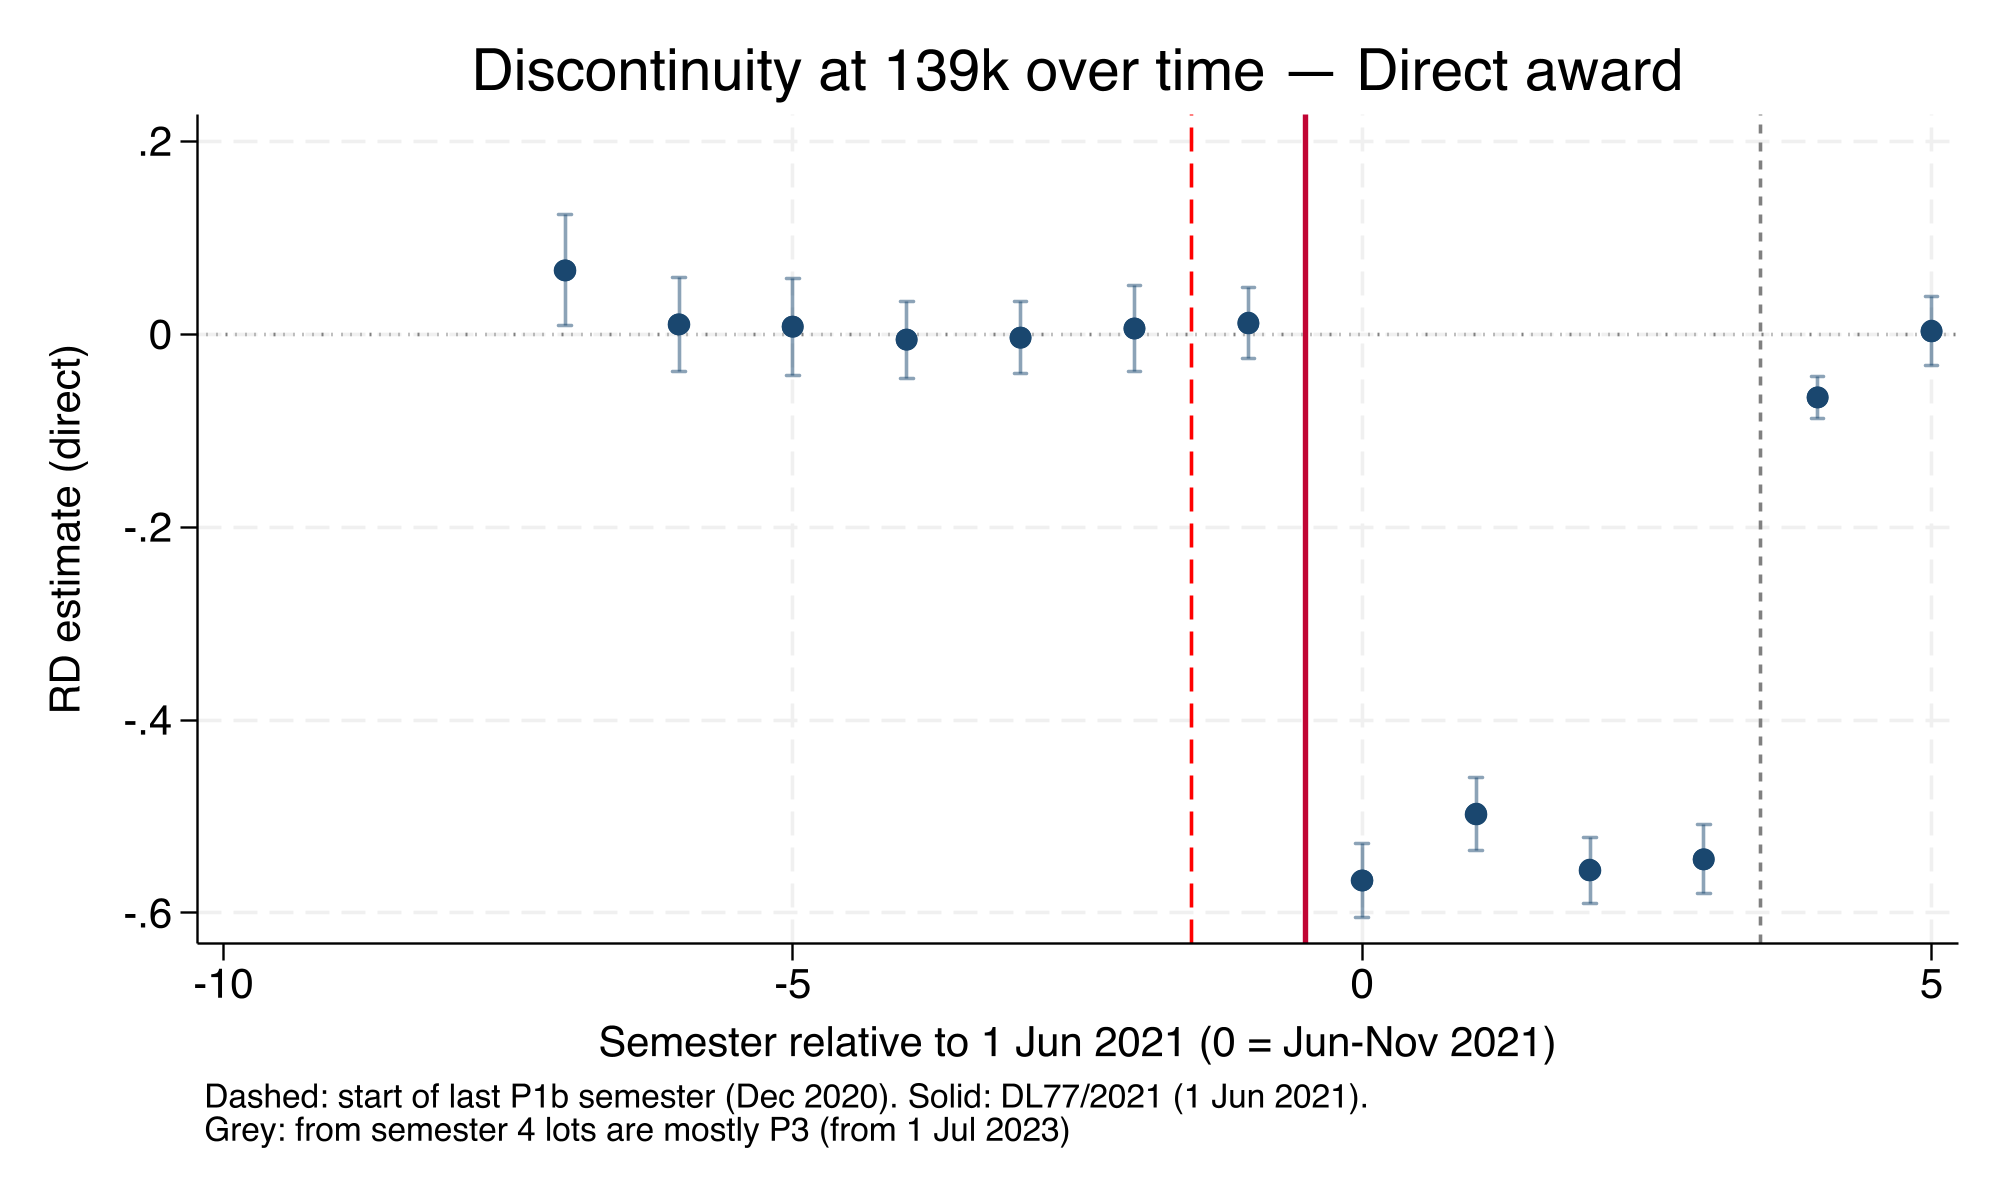
\includegraphics[width=0.78\textwidth]{M4_rd_direct_p1b.png}
\caption{Discontinuity in direct awards at \texteuro139k by semester (\code{rdrobust}, h = \texteuro20k). This figure retains the \code{rdrobust} convention, above minus below, so the reform is represented by a decline. Semester 0 is June--November 2021. The discontinuity emerges at the reform date and remains stable thereafter. From semester 4, lots fall under the new Code (P3). Code: \sect{4.5}.}
\label{fig:rdseries}
\end{figure}

Approximately 55\% of the long-run adjustment occurred in June 2021, the first month of implementation, and about 100\% by month 2 (Figure~\ref{fig:adjust}) \sect{6.1}. In the raw data, the direct-award share in the newly eligible band increased from 0.17 before the reform to 0.52 by month 2 and 0.60 in the long run. The corresponding share in the comparison band increased from 0.14 to 0.18.

\begin{figure}[H]
\centering
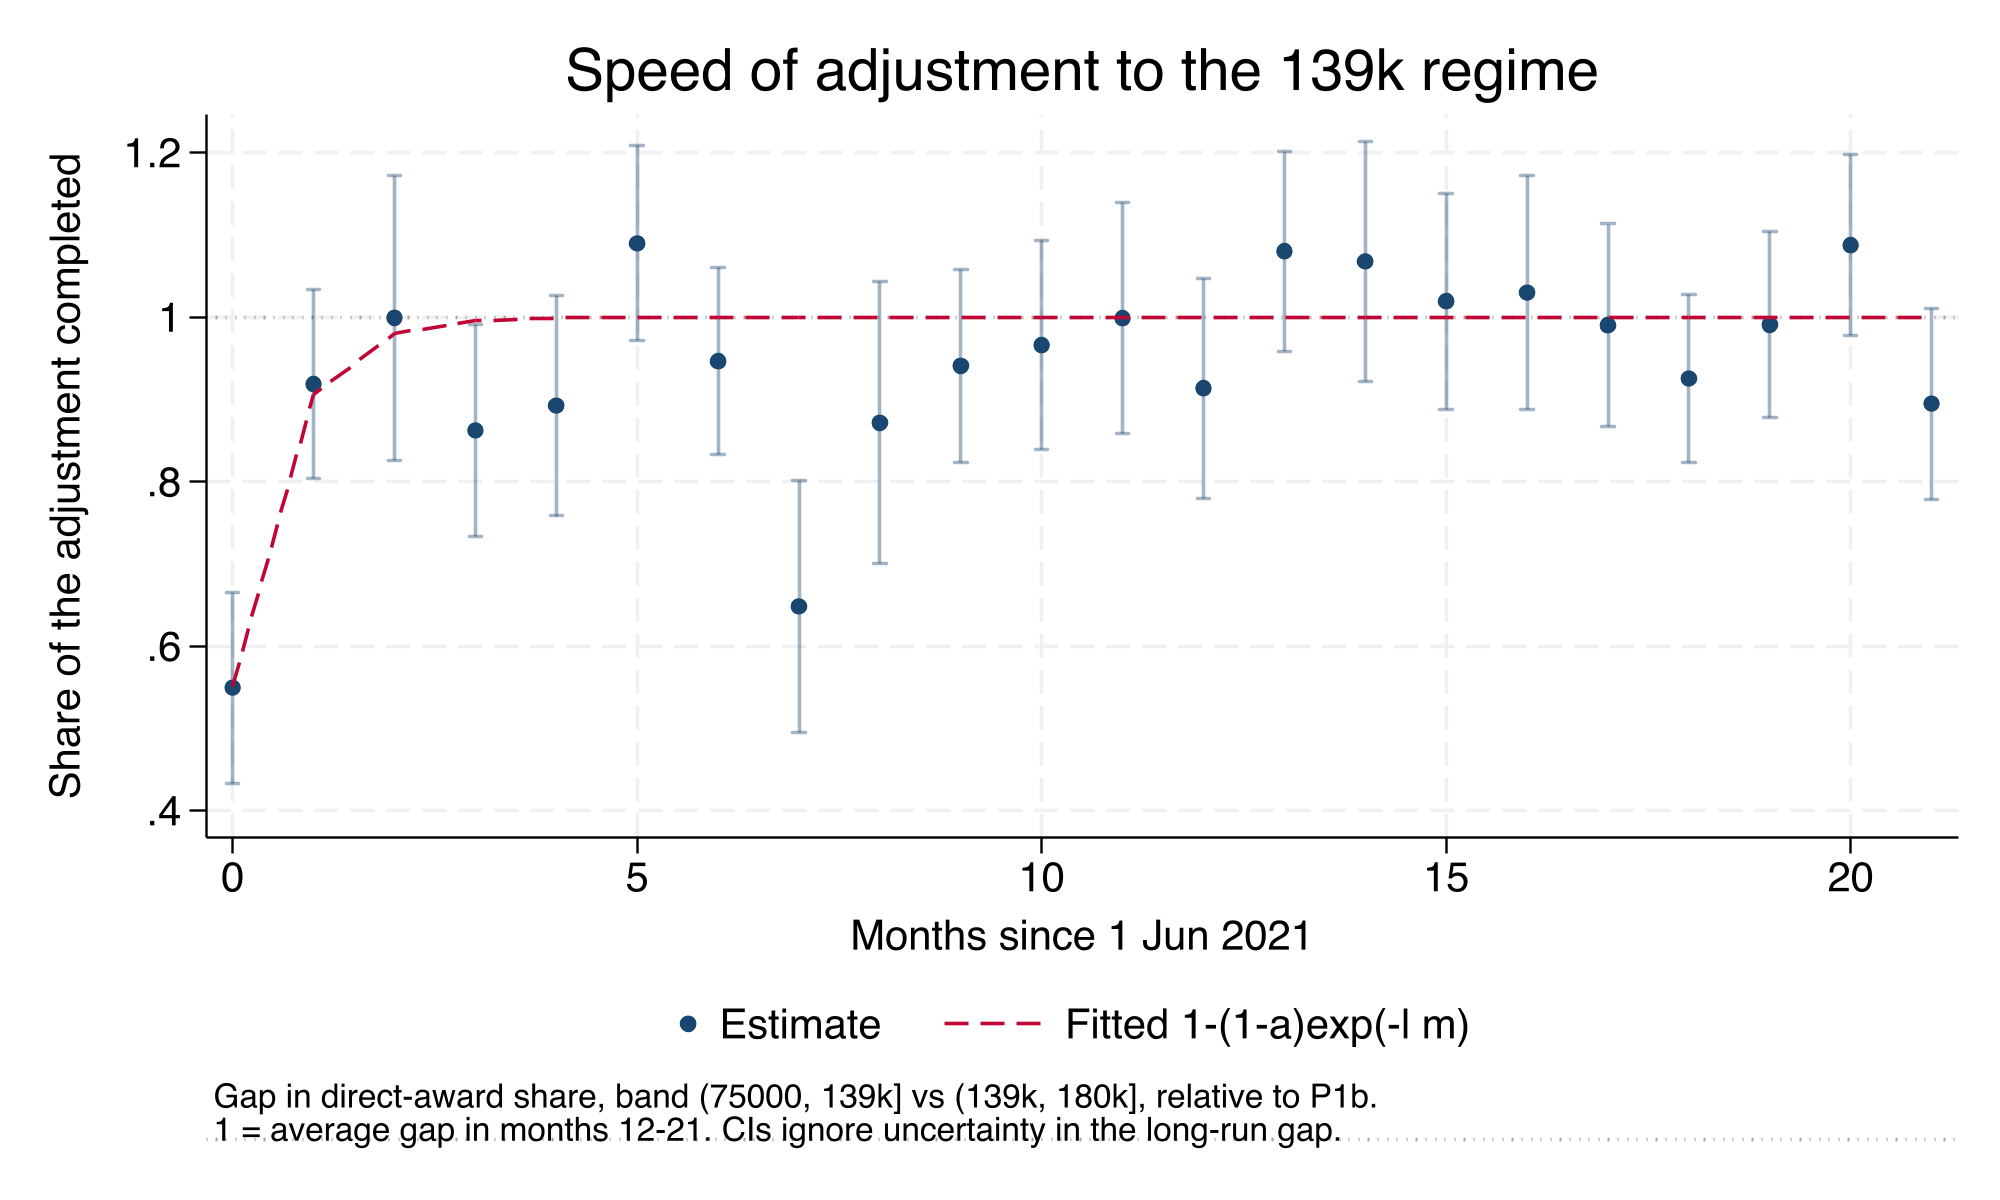
\includegraphics[width=0.72\textwidth]{S1_adjustment_curve_p1b.png}
\caption{Share of the long-run change completed, by month since 1 June 2021, with 95\% confidence intervals. Code: \sect{6.1}.}
\label{fig:adjust}
\end{figure}

The extent of adoption varies across regions, but there are no detectable regional differences in its speed \sect{6.2--6.4}. The standard deviation of regional take-up is 0.092, compared with an average sampling error of 0.043. Sectoral differences explain more variation than regional differences: the reported $R^2$ is 0.77 for sector, 0.55 for region and 0.86 when both are included. Region $\times$ sector interactions do not explain additional variation beyond sampling noise.

Take-up is lowest for medical supplies (CPV 33, 0.16), Sicily (0.12) and Molise. The highest take-up is observed in CPV sectors 71, 77 and 60, and in Friuli-Venezia Giulia, Veneto and Lombardy, where it is approximately 0.45.

\begin{table}[H]
\centering\small
\caption{Take-up and speed of adoption by region (sorted by take-up)}
\label{tab:regions}
\begin{tabular}{lrccc}
\toprule
Region & \makecell{Lots in band,\\P2} & \makecell{Long-run\\take-up} & \makecell{Share closed,\\months 0--2} & \makecell{Share closed,\\months 3--5} \\
\midrule
\tabinput{\tabdir/I_speed_regions_p1b.tex}
\bottomrule
\end{tabular}
\tabnote{Take-up is the long-run change in the direct-award gap between the eligible band (\texteuro75k--\texteuro139k) and the comparison band (\texteuro139k--\texteuro180k). Share closed is the gap in the indicated months divided by its long-run value; values above 1 indicate a temporary overshoot. Standard errors are in parentheses. ``Centrale'' denotes central authorities; ``Non classificato'' denotes authorities without a regional section. Code: \sect{6.2}.}
\end{table}

\begin{table}[H]
\centering\small
\caption{Adoption dynamics: specification checks}
\label{tab:speedchecks}
\begin{tabular}{lc}
\toprule
 & Change in gap \\
\midrule
\tabinput{\tabdir/I_speed_checks_p1b.tex}
\bottomrule
\end{tabular}
\tabnote{The two reported checks are expected to be close to zero. A third check compares take-up in two separate parts of the eligible band and yields a correlation of 0.79 across regions and across sectors. Code: \sect{6.5}.}
\end{table}

Adoption was rapid across regions, although its extent differed. The analysis does not distinguish between possible explanations for regional variation, such as administrative capacity, the composition of purchases or local procurement practices. The take-up measure is saved in \code{adjustment\_speed\_p1b.dta} for use as a moderator in subsequent analysis.

\section{Lot values and bunching below \texteuro139k}
\label{sec:bunching}

The bunching analysis examines whether authorities adjusted lot values to remain within the direct-award threshold. Figure~\ref{fig:bunching} compares the observed distribution with the fitted counterfactual in P1b and P2.

\begin{figure}[H]
\centering
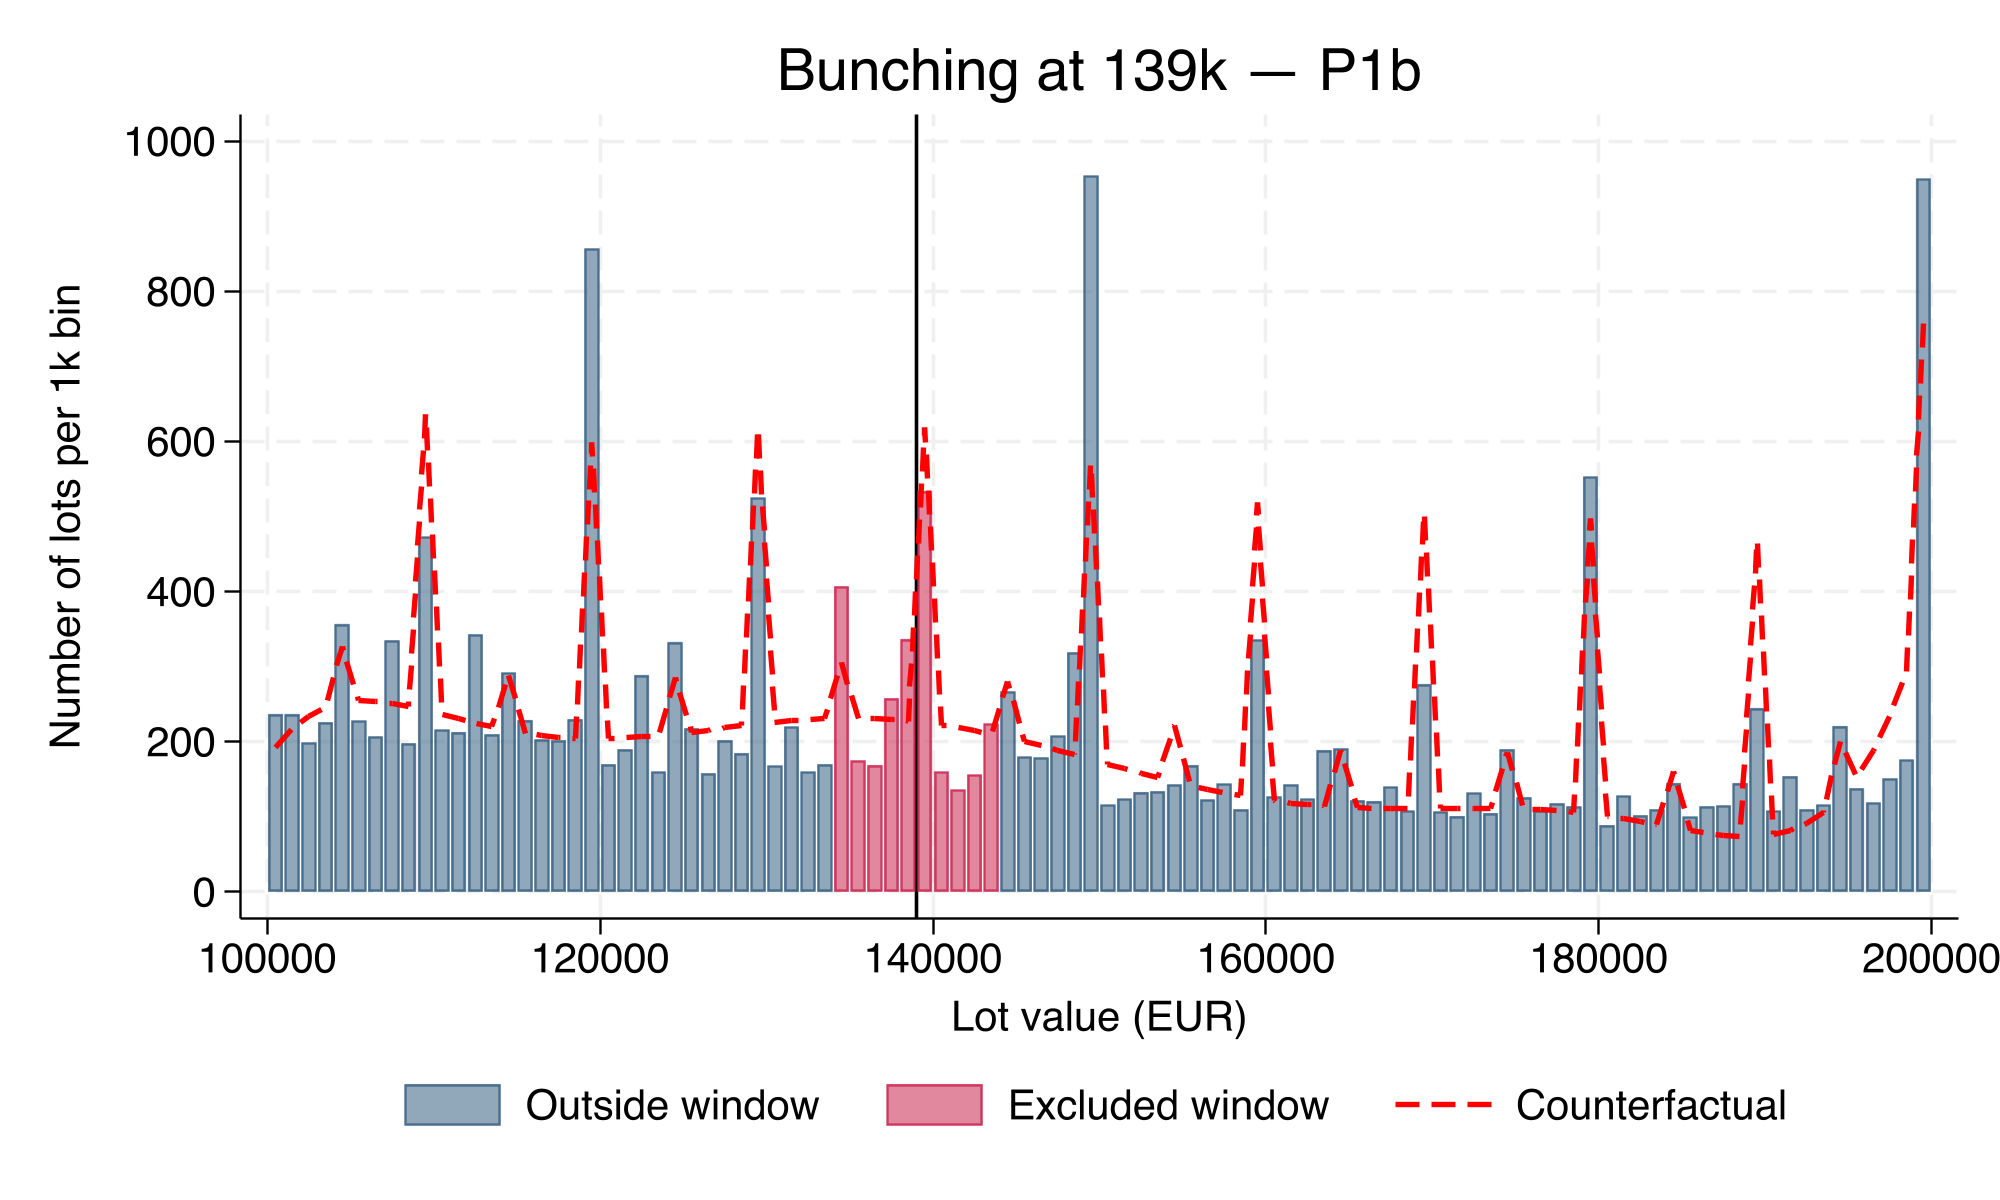
\includegraphics[width=0.49\textwidth]{B2_bunching_P1b.png}\hfill
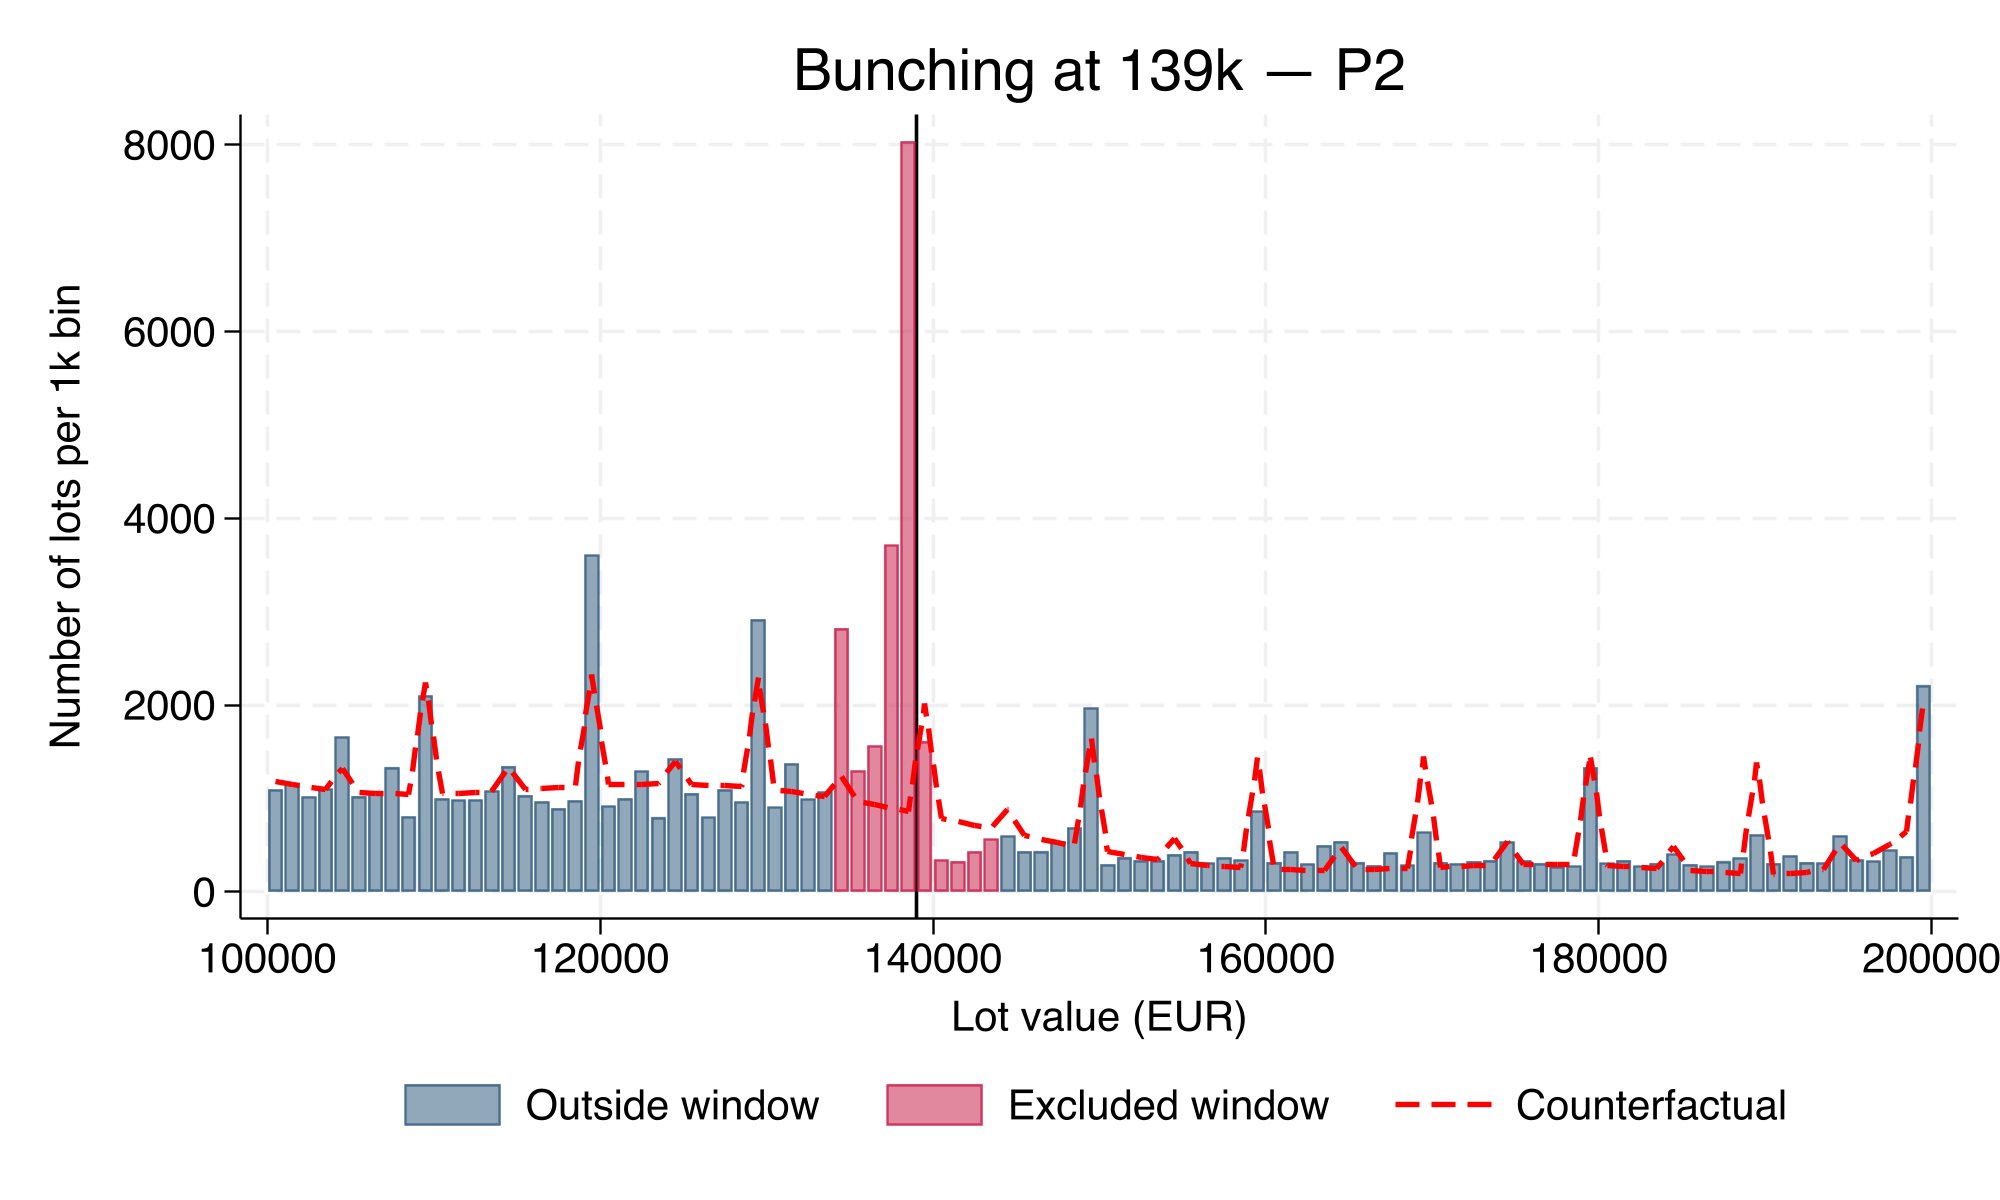
\includegraphics[width=0.49\textwidth]{B2_bunching_P2.png}
\caption{Lot counts per \texteuro1k bin and fitted counterfactual, P1b (left) and P2 (right). Code: \sect{3.2}.}
\label{fig:bunching}
\end{figure}

\begin{table}[H]
\centering\small
\caption{Excess mass just below \texteuro139k}
\label{tab:bunch}
\begin{tabular}{lccc}
\toprule
 & P2 & P1b & P2 $-$ P1b \\
\midrule
\tabinput{\tabdir/I_bunch_p1b.tex}
\bottomrule
\end{tabular}
\tabnote{95\% bootstrap percentile intervals in brackets (200 draws). Code: \sect{3.2--3.3}.}
\end{table}

\begin{table}[H]
\centering\small
\caption{Sensitivity of the excess mass to the specification}
\label{tab:bunchsens}
\begin{tabular}{lccc}
\toprule
Specification & P2 & P1b & P2 $-$ P1b \\
\midrule
\tabinput{\tabdir/I_bunch_sens_p1b.tex}
\bottomrule
\end{tabular}
\tabnote{``excl.'': width of the excluded window below or above the cutoff. Code: \sect{3.5}.}
\end{table}

In P2, the excess mass is $\hat b = 12.8$ (95\% interval 9.8--16.1): the additional lots in the five bins immediately below \texteuro139k are equivalent to the counterfactual count in approximately 13 bins of \texteuro1k. In P1b, the estimate is 0.5 (interval $-$0.6 to 1.8). The difference between the two periods, which is the estimate attributed to the reform, is 12.3 (interval 9.0--15.6). Across eight specifications, this difference ranges from 8.3 to 15.5.

The distribution also shifts between adjacent round values. The share of nearby lots valued at exactly \texteuro140{,}000 falls from 14.4\% to 3.9\%, while the share at exactly \texteuro139{,}000 rises from 3.2\% to 11.0\% \sect{3.4}.

Two separate calculations indicate where the additional lots come from \sect{3.5}. They use different benchmarks and should not be added together. The first remains within P2: if bunching consisted only of lots moved down from just above the cutoff, the excess below \texteuro139k would equal the shortfall relative to the fitted counterfactual just above it. The shortfall within \texteuro5k--\texteuro20k above the cutoff accounts for only 13--24\% of the P2 excess, depending on the width of the window used. The second compares the whole P2 distribution with P1b, after scaling each period by its number of lots in (\texteuro220k, \texteuro300k], a range the reform should not affect. Relative to P1b, P2 has 15.7k more lots in (\texteuro130k, \texteuro140k], 24.7k more in (\texteuro80k, \texteuro130k], 12.8k fewer in (\texteuro70k, \texteuro80k] and 5.5k fewer in (\texteuro140k, \texteuro220k]. The decline around \texteuro75k corresponds to the disappearance of bunching at the previous threshold. The 5.5k lots missing above \texteuro139k are about one-third of the 15.7k additional lots in the band just below; this ratio is an approximate comparison of two band counts, not a separate estimate, and it uses a wider window above the cutoff than the first calculation. Both calculations indicate that most of the additional lots below \texteuro139k did not come from just above the cutoff. The pattern is consistent with purchases previously kept below \texteuro75k being combined into larger lots, although the data do not identify individual purchases.

Table~\ref{tab:bunchgroups} reports excess mass by contract type, authority type and geographical area \sect{3.6}.

\begin{table}[H]
\centering\small
\caption{Excess mass by group}
\label{tab:bunchgroups}
\begin{tabular}{lcccc}
\toprule
Group & P2 & P1b & P2 $-$ P1b [95\% CI] & Gap vs reference [95\% CI] \\
\midrule
\tabinput{\tabdir/I_bunch_groups_p1b.tex}
\bottomrule
\end{tabular}
\tabnote{Same estimator in each group and period, 200 bootstrap draws each. Ten groups are compared without a multiple-testing correction. Code: \sect{3.6}.}
\end{table}

Bunching is observed in every group after the reform. It is weaker in the South than in the North, with a gap of $-$5.8, consistent with lower direct-award take-up in southern regions (Table~\ref{tab:regions}). It is also weaker for supplies than for services, with a gap of $-$4.2. Central authorities already exhibit bunching in P1b (4.9), providing further evidence, alongside Table~\ref{tab:design}, that \texteuro139k was relevant to their procurement decisions before the reform.

\section{The award process: speed, bids, price and criterion}

\begin{table}[H]
\centering\small
\caption{Award times and their components}
\label{tab:mainspeed}
\input{\tabdir/I_main_speed_p1b.tex}
\tabnote{Difference in discontinuities, h = \texteuro40k, awarded lots where both parts of the time are observed. Fixed effects CPV2 $\times$ post, region $\times$ post, year-month; SE clustered by authority in parentheses. Panel B instruments direct award with below $\times$ P2. Column 1 = column 2 + column 3, lot by lot and for the coefficients. * $p<0.10$, ** $p<0.05$, *** $p<0.01$. Code: \sect{4.2, 4.3, 4.8}.}
\end{table}

The ITT estimate for days to award is $-$52.3. Eligible lots near the cutoff were therefore awarded approximately 52 days earlier relative to lots just above it, net of the pre-reform difference. Compared with the control-period mean of 86 days below the cutoff, this represents a reduction of approximately 60\%.

The LATE estimate is $-$119 days, implying an award approximately four months earlier for lots that switched to direct award because of the reform. The ITT reduction comprises $-$15.4 days between publication and the bid deadline and $-$36.8 days between the deadline and the award. These changes are consistent with a procedure involving one firm and no tender evaluation; they do not, by themselves, indicate that award decisions were made in advance.

\begin{table}[H]
\centering\small
\caption{Awards recorded within 90 or 180 days: all lots}
\label{tab:selection}
\begin{tabular}{lcc}
\toprule
 & Award within 90 days & Award within 180 days \\
\midrule
\tabinput{\tabdir/I_selection_p1b.tex}
\bottomrule
\end{tabular}
\tabnote{All lots in the estimation window (N = 96{,}788), without conditioning on an award record. These outcomes combine the probability that an award is recorded with the timing of that award. Code: \sect{4.4}.}
\end{table}

These indicators are defined for every lot and therefore avoid conditioning the sample on the presence of an award record, although they remain sensitive to award reporting. Their estimates are consistent with the reduction in award times: eligible lots are approximately 10 percentage points more likely to have an award recorded within three months.

\begin{table}[H]
\centering\small
\caption{Bids, price and award criterion}
\label{tab:mainbids}
\input{\tabdir/I_main_bids_p1b.tex}
\tabnote{Same specification as Table~\ref{tab:mainspeed}, awarded lots; column 3 only lots whose award criterion is recorded. Log price ratio = log(award value / base value). * $p<0.10$, ** $p<0.05$, *** $p<0.01$. Code: \sect{4.2, 4.3, 4.8}.}
\end{table}

The coefficient on single-bid awards is +0.148, an increase of approximately 15 percentage points for eligible lots. This is largely mechanical: 87\% of direct awards in P2 record exactly one bid. The estimate therefore provides evidence of a procedural change, but is not an independent measure of reduced market competition.

The coefficient on the log price ratio is +0.075, corresponding to an approximate 7.5\% increase in the award-to-base-value ratio. The estimate loses statistical significance with a \texteuro5k donut, a local quadratic specification and a \texteuro20k bandwidth (Table~\ref{tab:robust}). Pre-reform coefficients also trend upwards in the value-band event study. Moreover, half of direct awards record an award value exactly equal to the base value. A higher ratio may therefore reflect the absence of a recorded discount rather than a higher price paid for a comparable purchase.

The coefficient on the MEAT criterion is $-$0.107: eligible lots are approximately 11 percentage points less likely to be awarded on the basis of the best price-quality ratio rather than the lowest price. Under ANAC indicator 1, this corresponds to a lower measured risk. However, the probability that the award criterion is recorded also falls by 12 percentage points below the cutoff (column 4). The MEAT estimates are therefore based on a selected sample and provide limited evidence about changes in discretion.

\section{Robustness and placebos (Part I)}

\begin{table}[H]
\centering\small
\caption{Robustness of the main estimates}
\label{tab:robust}
\begin{tabular}{lcccc}
\toprule
 & Direct award & Days to award & Log price ratio & Single bid \\
\midrule
\tabinput{\tabdir/I_robust_p1b.tex}
\bottomrule
\end{tabular}
\tabnote{Each row changes one element of the main specification. Donut specifications exclude lots within \texteuro1k / \texteuro2.5k / \texteuro5k of the cutoff. Authority size: log of the lots the authority published in the previous year, added as a control. Authority fixed effects: each authority's lots below the cutoff are compared with its own lots above. Strict eligibility assigns lots valued at exactly \texteuro139{,}000 to the above-threshold group, as the statute does; because these lots are predominantly direct awards, this reclassification reduces the estimates. rdrobust: P2 minus P1b, h = \texteuro20k, without fixed effects, with signs reversed. Value-band DiD: \texteuro100--130k versus \texteuro150--180k lots, P1b versus P2, without a running variable. Changes in band composition mean that this is a supplementary check. Direct awards are estimated on all lots; the remaining outcomes use lots with award records. Code: \sect{4.1, 4.2, 4.6, 4.7, 4.10}.}
\end{table}

\begin{table}[H]
\centering\small
\caption{Bandwidth sensitivity of the red-flag outcomes}
\label{tab:flagsrob}
\begin{tabular}{lcc}
\toprule
 & MEAT criterion & Days, deadline to award \\
\midrule
\tabinput{\tabdir/I_flags_robust_p1b.tex}
\bottomrule
\end{tabular}
\tabnote{Code: \sect{4.8}.}
\end{table}

\begin{table}[H]
\centering\small
\caption{Placebo cutoffs}
\label{tab:placebo}
\begin{tabular}{lccc}
\toprule
 & Direct award & Days to award & Log price ratio \\
\midrule
\tabinput{\tabdir/I_placebo_p1b.tex}
\bottomrule
\end{tabular}
\tabnote{Rows 1--4 use placebo cutoffs in P2 at values unaffected by the reform, restricting each estimation sample to one side of \texteuro139k (h = \texteuro15k; \texteuro10k at \texteuro200k). Rows 5--6 examine \texteuro139k before the reform. Coefficients are below minus above the placebo cutoff. Code: \sect{4.6c--d}.}
\end{table}

The first-stage and award-time results persist across specifications. The estimated reduction in days to award becomes smaller as the donut widens, suggesting that the effect is concentrated among lots immediately below \texteuro139k, where bunching is strongest. Controlling for authority size leaves all four estimates unchanged. With authority fixed effects, the first stage falls from 0.435 to 0.315, because the estimate now relies only on variation within authorities that have lots on both sides of the cutoff; the data do not show why the jump is smaller within authorities. The reduced-form estimates fall roughly in proportion: days to award $-$37.1 (SE 7.0), single bid +0.114, price ratio +0.047 ($p<0.05$). The implied effect per lot that switched procedure is therefore similar: $-$37.1/0.315 $\approx$ $-$118 days, against $-$52.3/0.435 $\approx$ $-$120 days in the main specification.

Direct-award discontinuities at the placebo cutoffs are small. The largest is 3.5 percentage points at \texteuro120k, where it is statistically significant, compared with 43.5 percentage points at the reform threshold. Award times, however, exhibit discontinuities at some placebo cutoffs and at \texteuro139k before the reform. Lots at exact round values, including \texteuro100{,}000 and \texteuro160{,}000, are awarded more quickly and fall on one side of these cutoffs. Excluding multiples of \texteuro5k approximately halves the placebo discontinuities. The difference-in-discontinuities design removes this pre-existing pattern to the extent that it remains stable across periods.

The price-ratio result is less robust. A discontinuity of $-$0.086 is also observed at the \texteuro160k placebo cutoff, reinforcing the uncertainty surrounding its interpretation.

\begin{figure}[H]
\centering
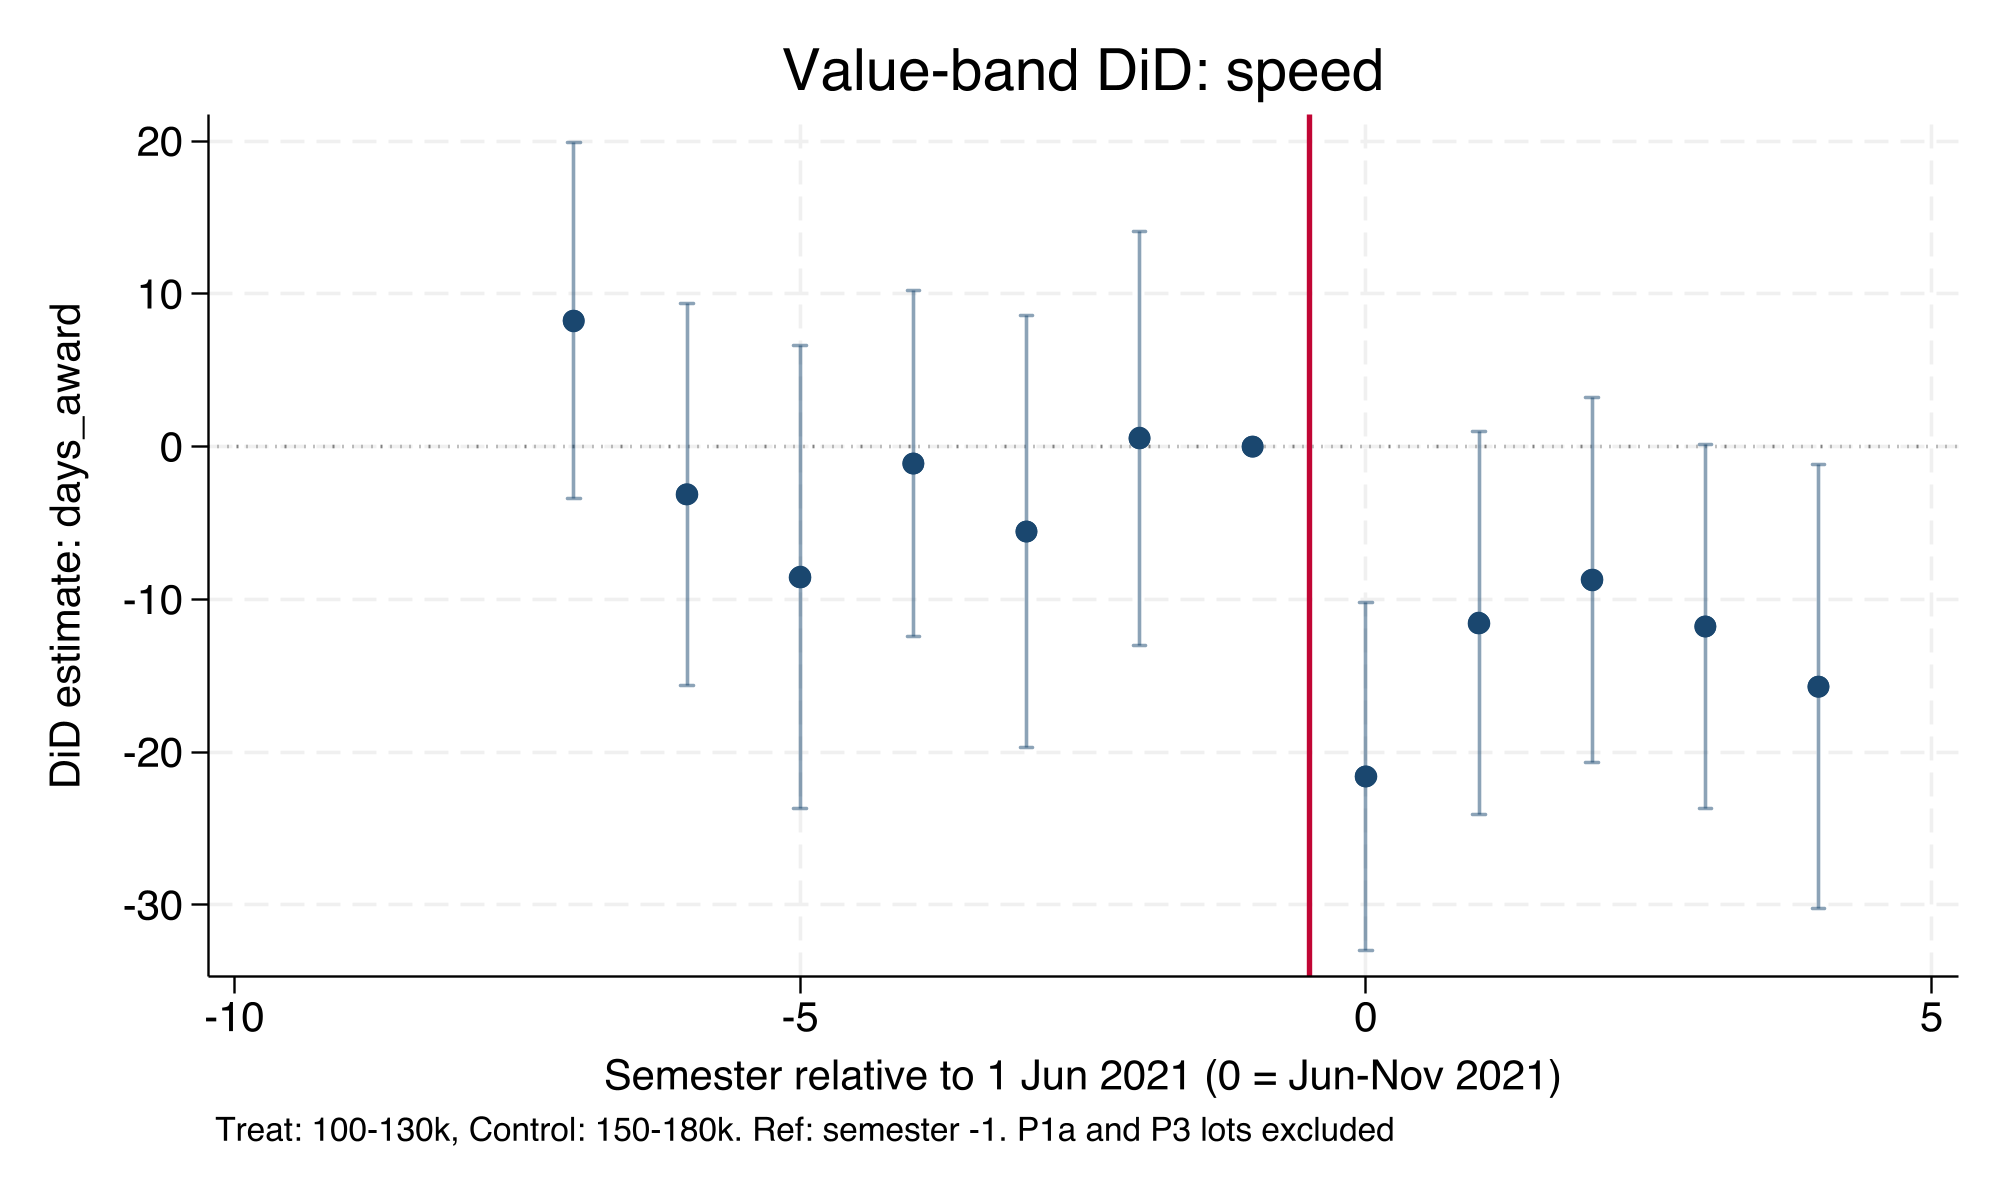
\includegraphics[width=0.7\textwidth]{M6_es_days_p1b.png}
\caption{Value-band DiD by semester, days to award (reference: last P1b semester). Pre-reform coefficients are small and not significant; after the reform eligible-band lots are awarded faster. Code: \sect{4.7}.}
\label{fig:esdays}
\end{figure}

\subsection*{Outcome cleaning}

Some outcome values are implausible or combine two different situations. Table~\ref{tab:cleancounts} counts them among the awarded lots of the estimation window \sect{4.9}. Award dates before the publication date affect 3.9\% of awarded lots. No lot has a bid deadline before publication, but 10.7\% of lots with both dates record the award before the bid deadline; most of these are direct awards, in which the ``deadline'' is a date set in the request to the chosen firm. About 1.1\% of lots record zero admitted bids and are coded as single-bid awards. The log price ratio has long tails: 2\% of lots fall outside its 1st and 99th percentiles.

\begin{table}[H]
\centering\small
\caption{Implausible or ambiguous outcome values (awarded lots in the estimation window)}
\label{tab:cleancounts}
\begin{tabular}{lrrr}
\toprule
Problem & Lots & Out of & Share \\
\midrule
\tabinput{\tabdir/I_cleaning_counts_p1b.tex}
\bottomrule
\end{tabular}
\tabnote{Code: \sect{4.9}.}
\end{table}

The main specification is not changed. Table~\ref{tab:cleaning} re-estimates the affected outcomes after removing these values, as an additional robustness check. The cleaning rules were fixed before the estimates were computed: lots with negative days to award are dropped; for the decomposition of award time, lots with a negative component are dropped; single-bid awards are set to missing when no admitted bid is recorded; and the price ratio is either trimmed or winsorized at its 1st and 99th percentiles.

\begin{table}[H]
\centering\small
\caption{Main estimates after outcome cleaning}
\label{tab:cleaning}
{\footnotesize\setlength{\tabcolsep}{4pt}%
\begin{tabular}{lccccc}
\toprule
 & Days to award & \makecell{Publication\\to deadline} & \makecell{Deadline\\to award} & Single bid & Log price ratio \\
\midrule
\tabinput{\tabdir/I_cleaning_p1b.tex}
\bottomrule
\end{tabular}}
\tabnote{Main specification. ``Cleaned'': negative durations dropped, single bid missing when no admitted bid is recorded, price ratio trimmed at its 1st and 99th percentiles. Last row: price ratio winsorized at the same percentiles. Code: \sect{4.9}.}
\end{table}

Dropping lots with negative durations reduces the estimated reduction in days to award from 52.3 to 43.2 days (SE 6.6) and the evaluation component from 36.8 to 31.4 days; the bid-window component is unchanged. Part of the main estimate therefore reflects award dates recorded before publication, which are more frequent among direct awards; the cleaned estimate remains large and precisely estimated. Recoding zero-bid lots leaves the single-bid estimate unchanged (0.152). Trimming the price ratio at its 1st and 99th percentiles reduces the coefficient from 0.075 to 0.050 but almost halves its standard error ($p<0.01$); winsorizing gives 0.065. The tails therefore add noise rather than drive the sign of the price result, but they do not resolve the other concerns about this outcome (specification sensitivity and recorded discounts).

\section{Summary of procedural and award-process results}

The evidence indicates rapid adoption of direct awards: the share immediately below \texteuro139k increased by approximately 44 percentage points, with adjustment largely completed within two months. The aggregate procedural discontinuity emerged at the reform date, although the pre-reform patterns for central authorities warrant separate consideration. Lot values shifted towards \texteuro139{,}000, and the wider distributional changes are consistent with smaller purchases being combined into larger lots. The lots that moved below the cutoff differ in observable characteristics from those above it, which the main specification partly absorbs through its sector and region fixed effects. Eligible contracts were awarded approximately 52 days earlier. Take-up was lowest in southern regions and medical supplies. Single-bid awards increased largely as a consequence of the procedure, while the price estimates remain too sensitive to the specification to support a firm conclusion.

%===============================================================================
\part*{Part II. Supplier selection and concentration}
\addcontentsline{toc}{section}{Part II. Supplier selection and concentration}
%===============================================================================

\section{Supplier selection}

This section examines whether greater scope for direct awards changed the allocation of contracts between established and new suppliers. The estimation follows the difference-in-discontinuities design in Part I and uses lots with an award record and a matched winner. Supplier histories include only contracts published on strictly earlier days, ensuring that different lots of the same tender are not treated as prior contracts relative to one another \sect{5.2}.

\begin{table}[H]
\centering\small
\caption{Supplier histories of contract winners}
\label{tab:mainwho}
{\footnotesize\setlength{\tabcolsep}{3.5pt}\input{\tabdir/II_main_p1b.tex}}
\tabnote{Columns: (1) no earlier contract with this authority in 24 months; (2--3) no public contract anywhere in 12 / 24 months; (4) won an earlier contract of this authority in 24 months; (5) same, same CPV3; (6) number of earlier contracts between the firm and the authority. Specification as in Table~\ref{tab:mainspeed}. * $p<0.10$, ** $p<0.05$, *** $p<0.01$. Code: \sect{5.3}.}
\end{table}

The probability that the winner is new to the authority increases by 0.056, or 5.6 percentage points, for eligible lots. The corresponding LATE is approximately 13 percentage points for lots that switched to direct award because of the reform.

The estimates for winners without any public contract in the preceding 12 and 24 months are +0.045 and +0.044, respectively. The increase is therefore not limited to firms that are new to an individual authority: eligible lots are also approximately 4.5 percentage points more likely to be awarded to firms without recent public-procurement activity anywhere in the observed data.

Repeat-winner coefficients are $-$0.042 across sectors and $-$0.043 within the same CPV3 sector. These estimates are only marginally significant ($p$ = 0.09 and 0.07), but are retained because they bear on the possibility that direct awards favour established suppliers. The coefficient on prior contracts is $-$2.0, indicating that winners of eligible lots have, on average, two fewer previous contracts with the authority.

\begin{table}[H]
\centering\small
\caption{Supplier-selection estimates: robustness and placebo tests}
\label{tab:whorob}
{\footnotesize\setlength{\tabcolsep}{4pt}%
\begin{tabular}{lccccc}
\toprule
 & New to authority & New to PP (12m) & New to PP (24m) & Repeat (24m) & Repeat (CPV3) \\
\midrule
\tabinput{\tabdir/II_robust_p1b.tex}
\bottomrule
\end{tabular}}
\tabnote{Authority fixed effects: each authority's lots below the cutoff are compared with its own lots above (Section~\ref{sec:balance}). Placebo rows: discontinuity at \texteuro139k in a pre-reform period alone (should be zero). Code: \sect{5.3}.}
\end{table}

All pre-reform placebo discontinuities at \texteuro139k are small and statistically insignificant. Using P0 as the control period yields coefficients of similar magnitude with greater precision. With authority fixed effects, which compare lots below and above the cutoff within the same authority (Section~\ref{sec:balance}), the estimates are 0.052 for new to the authority and 0.041 and 0.035 for new to public procurement, all significant at the 5\% level, and $-$0.038 for the two repeat-winner measures. Sorting of authorities across the cutoff therefore does not explain the shift towards new suppliers.

\section{Supplier concentration at the authority level}

The authority-level analysis examines whether the increased allocation of contracts to new firms is accompanied by lower supplier concentration. The conventional Herfindahl index (HHI) can decline mechanically as the number of contracts awarded within an authority-semester increases. This matters because exposed authorities awarded approximately 25\% more lots after the reform.

The analysis therefore also uses $S$, the probability that two distinct contracts within the same authority-semester were awarded to the same firm. This measure removes the mechanical dependence on the number of contracts. For $k$ contracts drawn at random from the cell, the expected HHI is exactly $1/k + (1-1/k)\,S$ \sect{5.4b}.

\begin{table}[H]
\centering\small
\caption{Concentration: exposure $\times$ post}
\label{tab:conc}
\begin{tabular}{lc}
\toprule
 & Exposure $\times$ post \\
\midrule
\tabinput{\tabdir/II_concentration_p1b.tex}
\bottomrule
\end{tabular}
\tabnote{Authority $\times$ semester panel, P1b and P2, authority and semester fixed effects, SE clustered by authority. 18{,}907 cells, 3{,}229 authorities; mean exposure 0.16. The last two rows are coefficients of an event study of $S$ (reference: last P1b semester). Code: \sect{5.4, 5.4b}.}
\end{table}

The coefficient for the value-based HHI is $-$0.071. Moving from zero exposure to the sample mean of 0.16 therefore corresponds to an HHI reduction of approximately 0.011. Much of the apparent decline in concentration is associated with the number of contracts: the count-based HHI coefficient is $-$0.113 across all cells, but $-$0.050 among cells with at least two contracts.

The coefficient for $S$ is $-$0.038, indicating a smaller decline after removing the mechanical effect of contract counts. At mean exposure, the probability that two contracts from the same authority go to the same firm falls by approximately 0.006, equivalent to 17\% of its mean of 0.036. The event study shows no pre-reform gap in semester $-2$, and the decline is concentrated in the first semester after the reform.

The coefficient on the share of firms new to the authority is +0.096, consistent with the lot-level estimates in Table~\ref{tab:mainwho}.

\section{Summary of supplier-selection and concentration results}

Lots that became eligible for direct award were more likely to be awarded to firms without a recent contract with the authority. A similar increase is observed for firms without any recent public contract in the available data. The estimates therefore provide no evidence that authorities used the additional discretion to increase awards to established suppliers. At the authority level, the decline in concentration is small after accounting for the increase in contract counts.

%===============================================================================
\part*{Part III. Supplier networks and market entry}
\addcontentsline{toc}{section}{Part III. Supplier networks and market entry}
%===============================================================================

\section{Network classification and supplier histories}

The increase in awards to firms new to the authority may reflect entry by firms without recent activity in the relevant market, or rotation among firms already connected to the authority through its supplier network. A related possibility is the return of a former supplier after an intervening award to another firm, consistent with the \textit{principio di rotazione}.

The network measures are constructed in Python in \code{code/net\_py/} and run through \code{code/net\_master.do} \sect{7}. For each lot awarded to firm $f$ by authority $a$, the classification uses awards in the same CPV2 market during the preceding 24 months. Only strictly earlier award dates are included, with historical data available from 2015. Each winner is assigned to one of five mutually exclusive classes:
\begin{itemize}
\item \textbf{Incumbent}: $f$ won $a$'s most recent award in the same CPV3 sector as the current lot (if several awards share that date, any of their winners counts).
\item \textbf{Prior supplier}: $f$ won at least one award from $a$ in the CPV2 market during the history window, in any CPV3 sector, but is not the incumbent.
\item \textbf{Indirectly connected supplier}: $f$ did not supply $a$, but another authority purchased from both $f$ and one of $a$'s suppliers.
\item \textbf{Outsider}: $f$ won awards elsewhere in the market but has no such connection to $a$.
\item \textbf{New to the market}: $f$ won no award in the market during the history window.
\end{itemize}

The \emph{return after a gap} indicator is not a sixth class. It equals one when $f$ won at least one earlier award from $a$ \emph{in the same CPV3 sector as the current lot} during the window, but did not win $a$'s most recent award in that sector. It is therefore a subset of the prior-supplier class: prior suppliers whose earlier relationship with the authority was in the same narrow sector, which is the situation that the rotation principle addresses. Prior suppliers whose earlier awards were only in other CPV3 sectors of the same market are not counted as returns. This explains why the two indicators have different means (0.319 and 0.296 below the cutoff in P1b) and different coefficients. The five class indicators sum to one for every lot; their estimated coefficients consequently sum to zero, as verified in the code.

\begin{figure}[H]
\centering
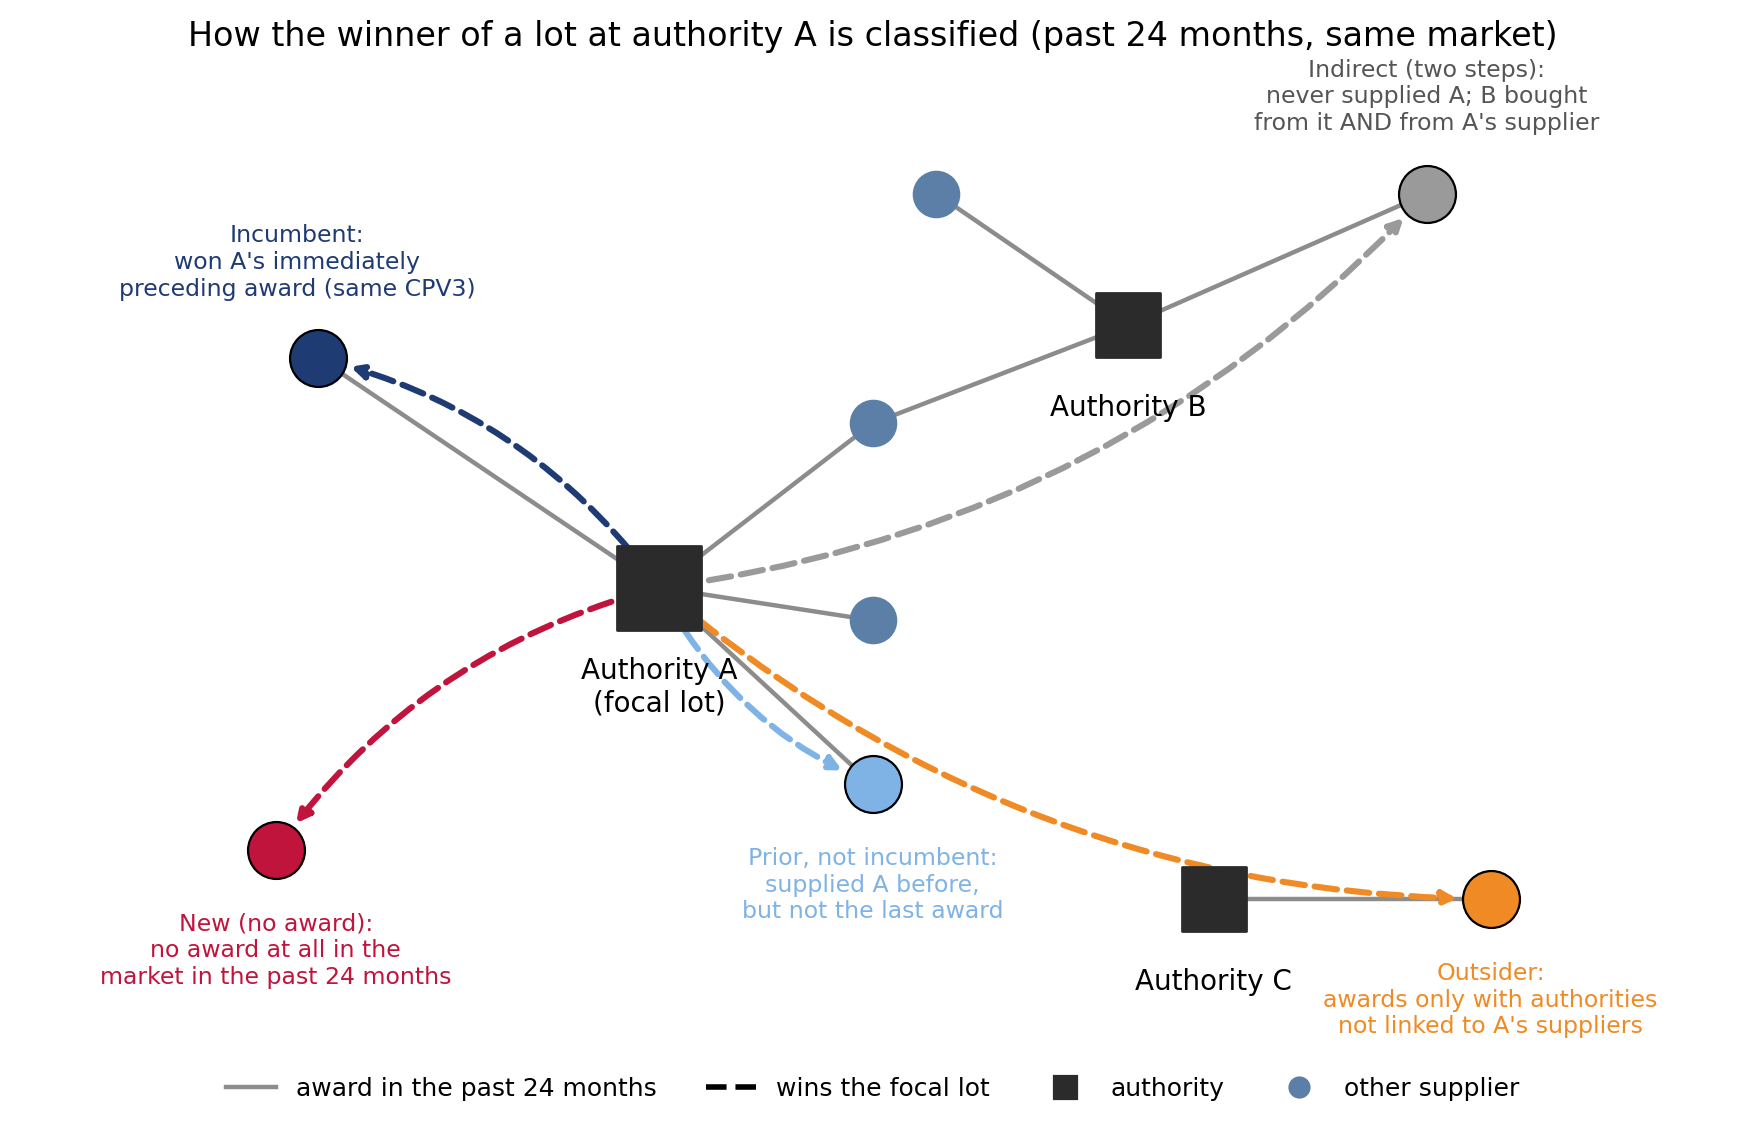
\includegraphics[width=0.62\textwidth]{net_graph_schematic.png}
\caption{Schematic of the winner classes. Code: \code{code/net\_py/net\_fig\_graphs.py}.}
\label{fig:schematic}
\end{figure}

\section{Network results}

\begin{table}[H]
\centering\small
\caption{Contract winners by network position and market history}
\label{tab:mainnet}
\input{\tabdir/III_main_p1b.tex}
\tabnote{Difference in discontinuities, specification as in Part II, lots with a winner. The indirect and outsider classes and the winner's log degree are not shown (Section~\ref{sec:dropped}). * $p<0.10$, ** $p<0.05$, *** $p<0.01$. Code: \sect{7.2}.}
\end{table}

The coefficient for winners new to the market is +0.050. Eligible lots are therefore 5 percentage points more likely to be awarded to a firm with no award in that market during the preceding 24 months. The corresponding LATE is approximately 11 percentage points. Below the cutoff, the raw share increases from about 0.21 to 0.27.

The coefficient for prior suppliers is $-$0.050, indicating a decline in awards to firms that previously supplied the authority but did not win its most recent contract in the same sector. The incumbent coefficient is $-$0.012 and statistically insignificant, providing no evidence of an increase in awards to the most recent winner. The return-after-a-gap coefficient is also negative, at $-$0.036 ($p$ = 0.09). Returns by former suppliers in the same sector therefore do not become more frequent; the estimate instead suggests a possible decline.

\begin{figure}[H]
\centering
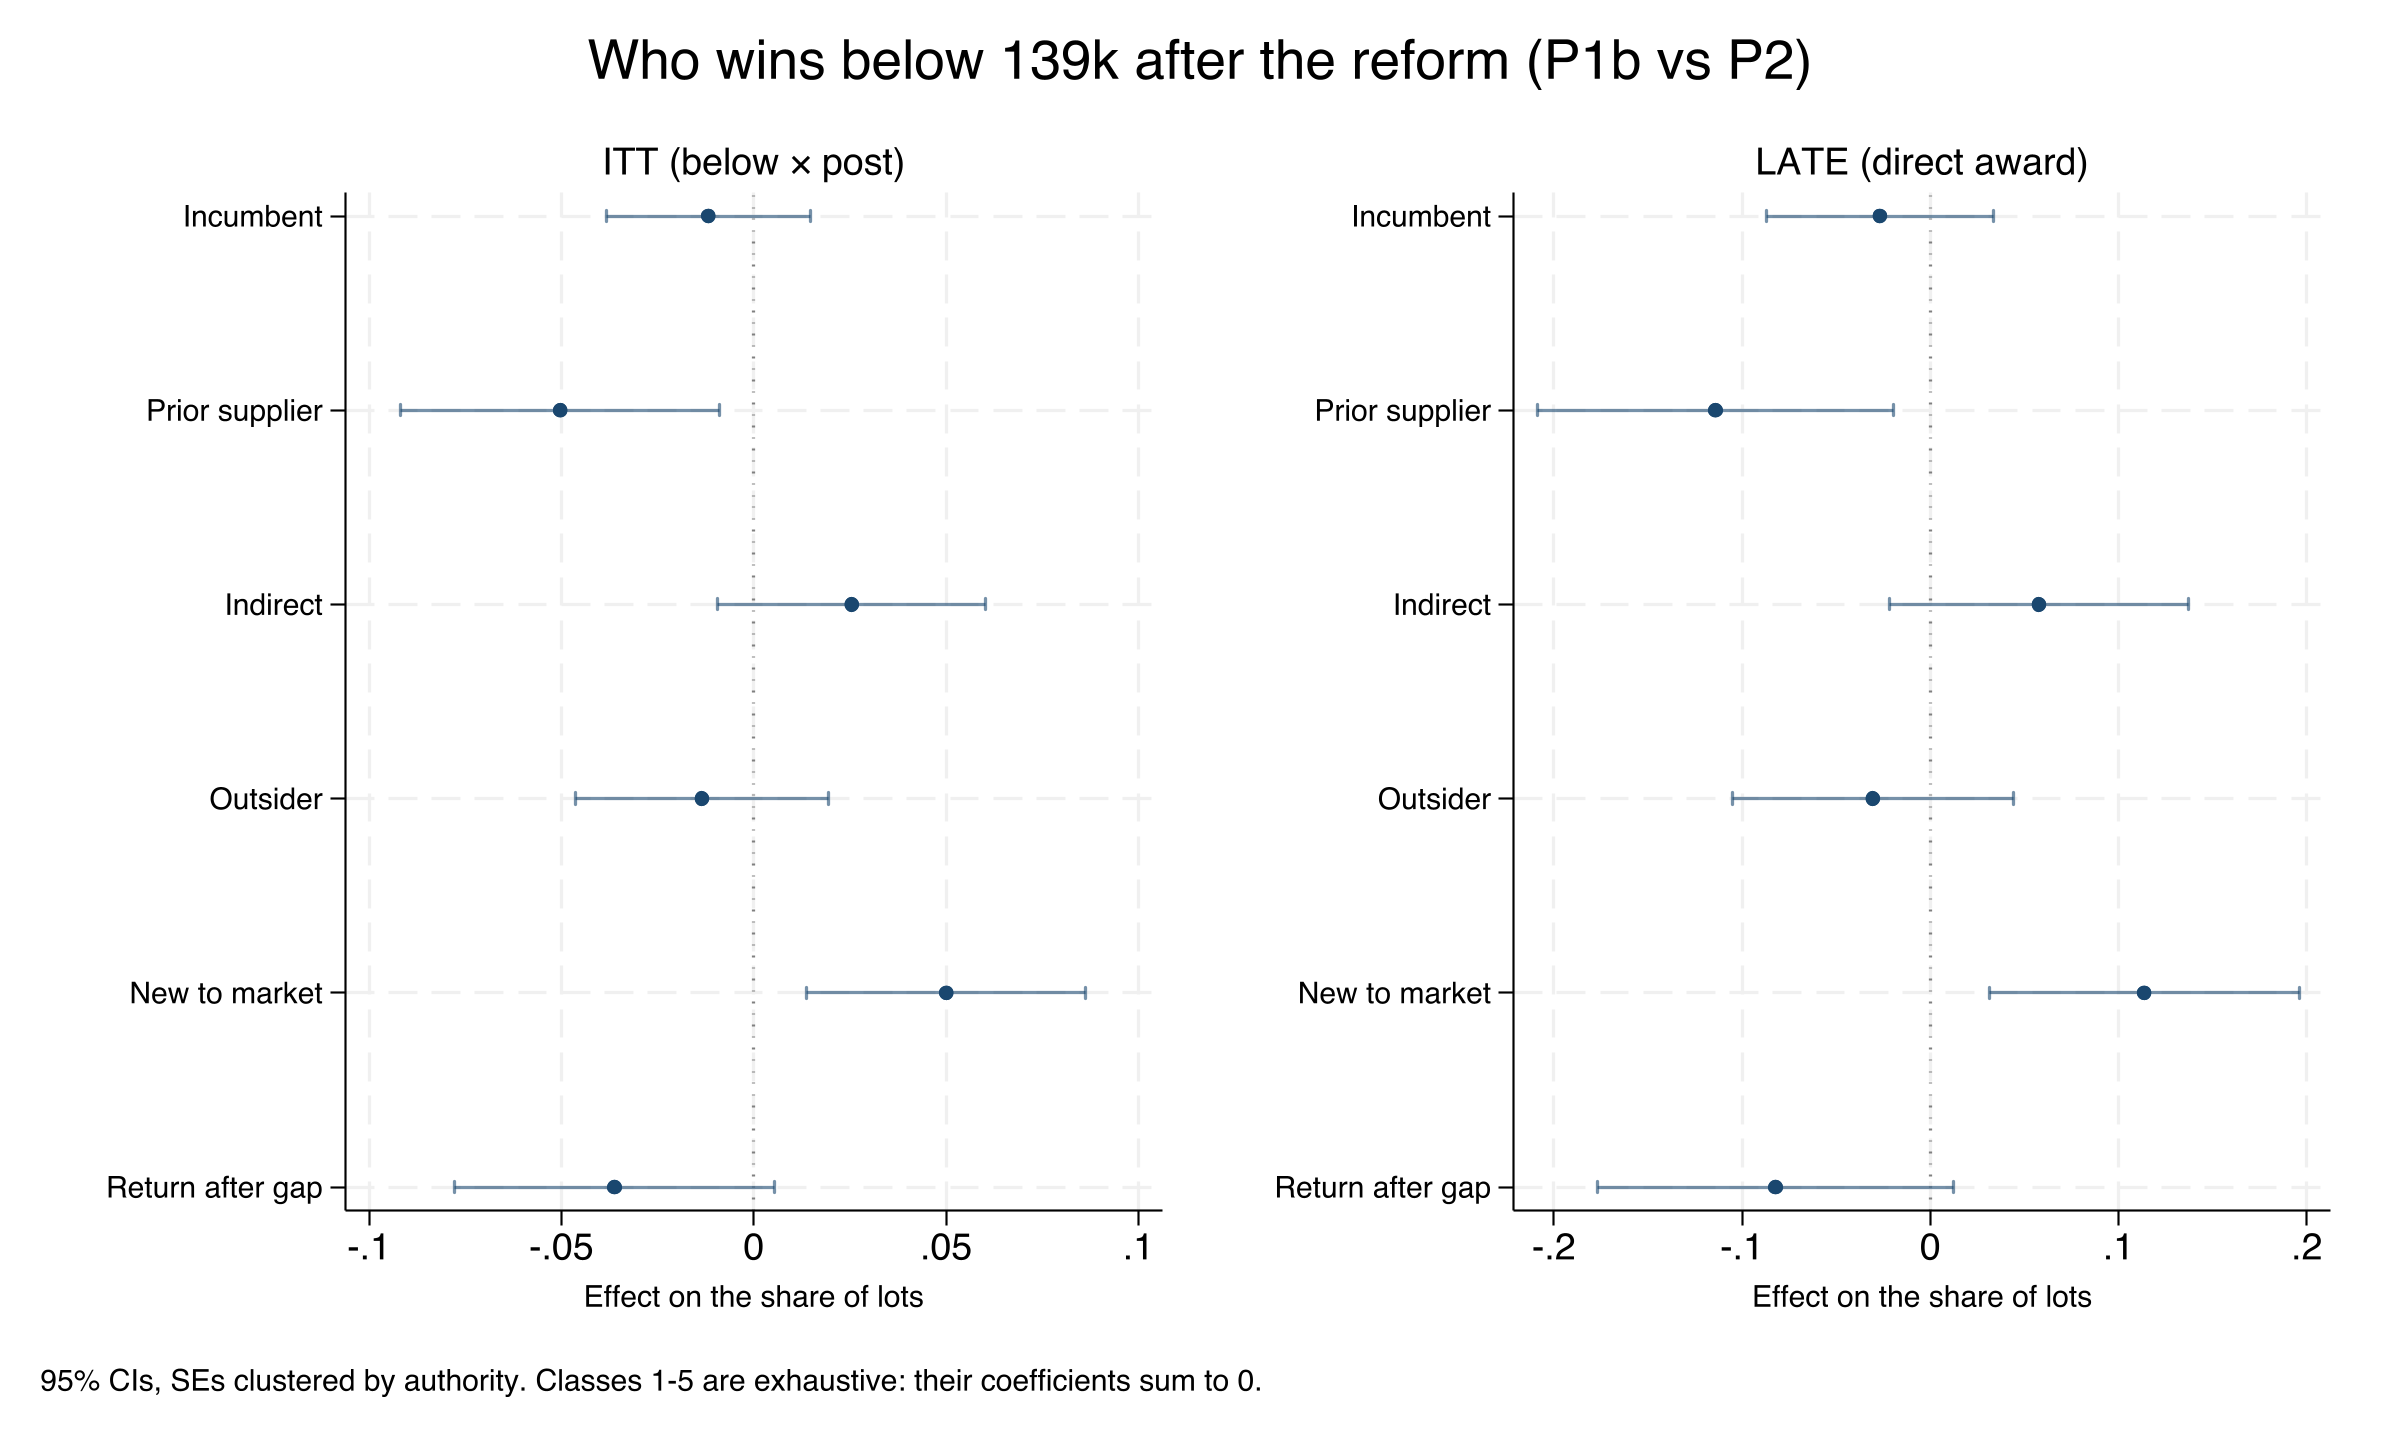
\includegraphics[width=0.9\textwidth]{N2_network_coef_p1b.png}
\caption{ITT and LATE for the five classes and return after a gap, with 95\% intervals. Code: \sect{7.5}.}
\label{fig:netcoef}
\end{figure}

\begin{table}[H]
\centering\small
\caption{Network classes: robustness}
\label{tab:netrob}
\begin{tabular}{lcccc}
\toprule
 & New to market & Prior supplier & Incumbent & Return after gap \\
\midrule
\tabinput{\tabdir/III_robust_p1b.tex}
\bottomrule
\end{tabular}
\tabnote{Authority fixed effects: within-authority comparison (Section~\ref{sec:balance}). 12-month window: shorter history, so more firms count as new in both periods. Network fixed before the reform: classes built only from awards between 17 July 2018 and 16 July 2020. Code: \sect{7.3}.}
\end{table}

\begin{table}[H]
\centering\small
\caption{Network classes: placebos}
\label{tab:netplac}
\begin{tabular}{lcccc}
\toprule
 & New to market & Prior supplier & Incumbent & Return after gap \\
\midrule
\tabinput{\tabdir/III_placebo_p1b.tex}
\bottomrule
\end{tabular}
\tabnote{The initial \texteuro120k placebo is nonzero. Lots valued at exactly \texteuro120{,}000 are more likely to be awarded to new firms than nearby lots (0.340 versus 0.262), and are assigned to the above-cutoff group in this placebo. Excluding these observations, or all multiples of \texteuro5k, eliminates the placebo discontinuity. Code: \sect{7.4}.}
\end{table}

The coefficient for winners new to the market is statistically significant in almost all specifications. It remains significant across the bandwidth choices except \texteuro20k, where $p$ = 0.09, and under donut specifications, exclusion of lots valued at exactly \texteuro139{,}000, exclusion of all round values, a network fixed before the reform, CPV3 market definitions, P0 as the control period and value-band DiD. The estimate is weaker with a 12-month history window. With authority fixed effects the new-to-the-market coefficient is 0.038 ($p<0.05$) and the prior-supplier coefficient $-$0.056 ($p<0.01$); the incumbent coefficient remains close to zero.

Pre-reform placebo tests at \texteuro139k do not reveal significant discontinuities. The only reported placebo failure, at \texteuro120k, disappears when observations at the exact round value are excluded.

\section{Summary of network results}

The estimates are more consistent with increased awards to firms without recent activity in the market than with rotation among suppliers already known to the authority. Firms new to the market account for most of the increase in new winners, and former suppliers do not return more frequently. The data do not establish whether awards to indirectly connected suppliers or outsiders declined, since the estimates for these classes are inconclusive. Rotation rules applied on both sides of the cutoff in P2 (Section~\ref{sec:law}), so they do not by themselves explain the difference between eligible and ineligible lots, although the form of rotation differed between direct awards and negotiated procedures.

%===============================================================================
\section{Assessment of the evidence}
%===============================================================================

\begin{table}[H]
\centering\small
\caption{Findings and strength of the evidence}
\label{tab:claims}
\begin{tabularx}{\textwidth}{>{\raggedright}p{5.2cm}>{\raggedright}p{2.6cm}X}
\toprule
Claim & Evidence & Main support \\
\midrule
The reform increased direct awards at \texteuro139k & Strong & First stage 0.435; small aggregate pre-reform discontinuity, with an exception for central authorities; adoption within two months \\
Lot values shifted towards eligibility & Strong & Excess mass 12.8 in P2 against 0.5 in P1b; concentration shifted from \texteuro140k to \texteuro139k; bunching in every group \\
Lots on the two sides remain comparable & Partly & Sector, region, authority type and authority size change at the cutoff after the reform; sector and region are absorbed by the main fixed effects; results hold with authority fixed effects, with smaller reduced-form estimates \\
Awards were recorded sooner & Strong & $-$52 days ITT, $-$119 LATE; $-$43 days after removing negative durations; $-$37 days with authority fixed effects; all-lot outcomes are consistent \\
More contracts were awarded to new firms & Moderate to strong & +0.045 to +0.056 across three definitions; similar with P0 and with authority fixed effects; placebos pass after accounting for round values \\
Increased rotation among known suppliers & Not supported & Prior suppliers $-$0.050; no increase in incumbent awards or returns \\
Greater frequency of single-bid awards & Observed; largely mechanical & Direct awards generally record one bid \\
Higher award-to-base-value ratios & Inconclusive & Log-ratio coefficient +0.075; sensitive to specification and recording practices \\
Lower supplier concentration & Weak & Fixed-size measure $-$0.038; sensitive to sample restrictions \\
Greater discretion through the award criterion & Not supported & MEAT $-$0.107 in a selected sample \\
\bottomrule
\end{tabularx}
\end{table}

%===============================================================================
\section{Results not shown in the main tables}
\label{sec:dropped}
%===============================================================================

\begin{table}[H]
\centering\small
\caption{Estimates excluded from the main tables}
\label{tab:dropped}
\begin{tabular}{lc}
\toprule
 & Estimate \\
\midrule
\tabinput{\tabdir/X_dropped_p1b.tex}
\bottomrule
\end{tabular}
\tabnote{Estimates from the main specification. The reasons for exclusion are discussed below.}
\end{table}

\begin{itemize}
\item The number of bids is replaced by the single-bid indicator as a clearer measure of the procedural change. Both outcomes are mechanically affected by direct awards.
\item The number of invited firms is statistically insignificant and sensitive to extreme observations.
\item The estimate of $S$ for cells with at least five contracts is statistically insignificant. It is retained here because it indicates that the concentration result is sensitive to sample restrictions.
\item The indirectly connected and outsider classes yield statistically insignificant estimates. Their signs differ across control periods and between the regressions and the raw binned plots.
\item The winner's log degree is mechanically related to market entry because firms new to the market have degree zero. It is replaced by the new-to-the-market indicator.
\end{itemize}

Several analyses were excluded earlier and were not re-estimated. Market-level concentration, defined at CPV3 $\times$ province $\times$ year, had limited statistical power because the median market contained only two lots per year. The price-ratio event study exhibited pre-reform drift. The authority-level network panel produced a null result with P1b and did not permit a pre-trend test. Finally, the winner's number of client authorities was initially computed over the full data window, including subsequent years. This measure was replaced by log degree over the preceding 24 months, which was itself subsequently excluded for the reason given above.

%===============================================================================
\section{Data limitations and specification decisions}
\label{sec:limits}
%===============================================================================

The main estimates use the outcomes as recorded. The outcome-cleaning tables in Part I quantify the main data problems (negative durations, zero admitted bids coded as single-bid awards and the tails of the price ratio) and report cleaned estimates as robustness checks only.

Lot values are nominal. This is appropriate for the main design, because the legal threshold is itself a nominal amount, and the price ratio has no unit. Nominal values matter only for comparisons of the whole value distribution across periods (Section~\ref{sec:bunching}) and for the value-weighted HHI. Inflation in 2022 would shift lot values upwards, which is the opposite direction to the observed movement of lots towards \texteuro139k from above.

Authority legal types come from a 2026 snapshot of the ANAC register. The register contains one record per authority with the dates on which the record was created and closed, but no history of changes in legal type. The classification therefore reflects current legal types and may misclassify authorities that changed form between 2020 and 2023.

P0 is used only in the alternative-control specifications; the complete analysis has not been rerun using \code{global CTRL "P0"}.

Several specification choices were made after inspecting the results and are documented in the Deviations section of \code{pilot\_report.md}. These include replacing P0 with P1b as the control period, classifying lots valued at exactly \texteuro139{,}000 as eligible although the statute uses a strict threshold, selecting the bunching dummies and estimation window, and restricting supplier histories to strictly earlier days. Red-flag outcomes, fixed-size concentration, bunching by group and new-to-public-procurement outcomes were added on 13--14 November. The balance test, the authority fixed-effects rows and the outcome-cleaning checks were added on 14 November.

\appendix
\section{Project files and reproducibility}

\begin{table}[H]
\centering\small
\begin{tabularx}{\textwidth}{>{\raggedright}p{5cm}>{\raggedright\arraybackslash}X}
\toprule
Component & File \\
\midrule
Main code (Parts 1--8) & \code{code/full\_analysis\_commented.do} \\
Complete analysis workflow & \code{code/00\_master.do} \\
Network build (Python) & \code{code/net\_master.do}, \code{code/net\_py/}; notes in \code{docs/net\_build\_note.md} \\
Execution log & \code{code/logs/full\_analysis\_commented\_p1b.log} \\
Consolidated coefficient estimates & \code{results/tables/coefficients\_p1b.csv} \\
Report tables & \code{results/tables/tex/} (written by Part 8) \\
Figures & \code{results/figures/} \\
Legal texts & \code{data/raw/law/} \\
Results in Markdown & \code{results/report.md} \\
Decisions and deviations & \code{pilot\_report.md} \\
\bottomrule
\end{tabularx}
\end{table}

\end{document}
